
\begin{figure}[!htb]
\centering

\begin{tabular}{cccccccccc}
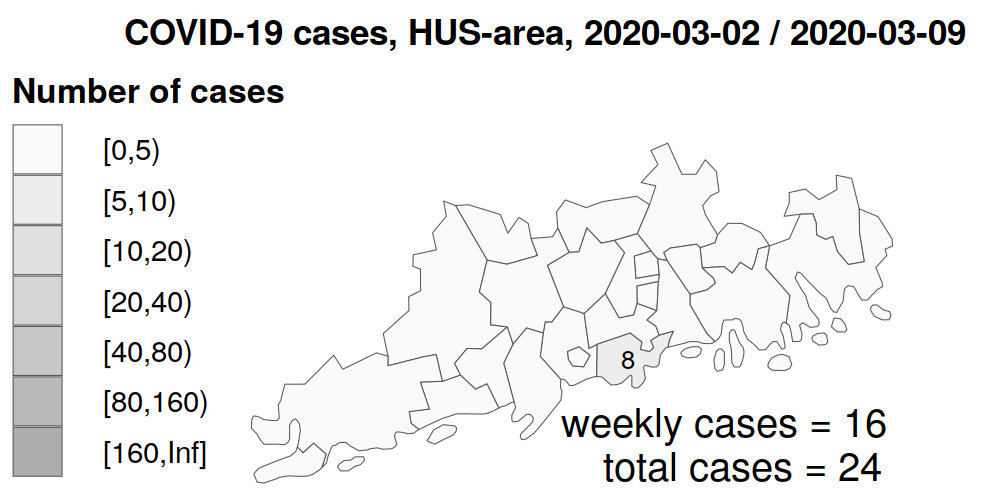
\includegraphics[width = 2.1in]{img/hus_incidence_04.png} & 
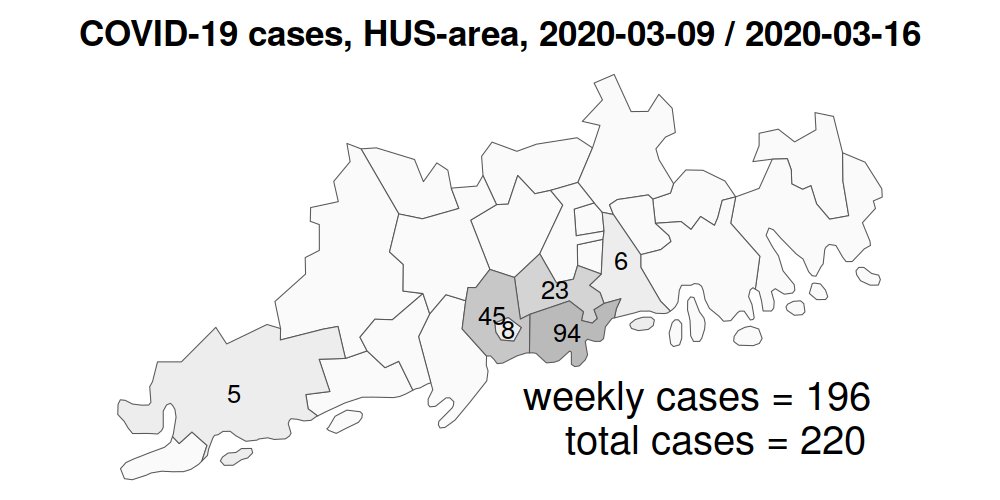
\includegraphics[width = 2.1in]{img/hus_incidence_05.png} &  
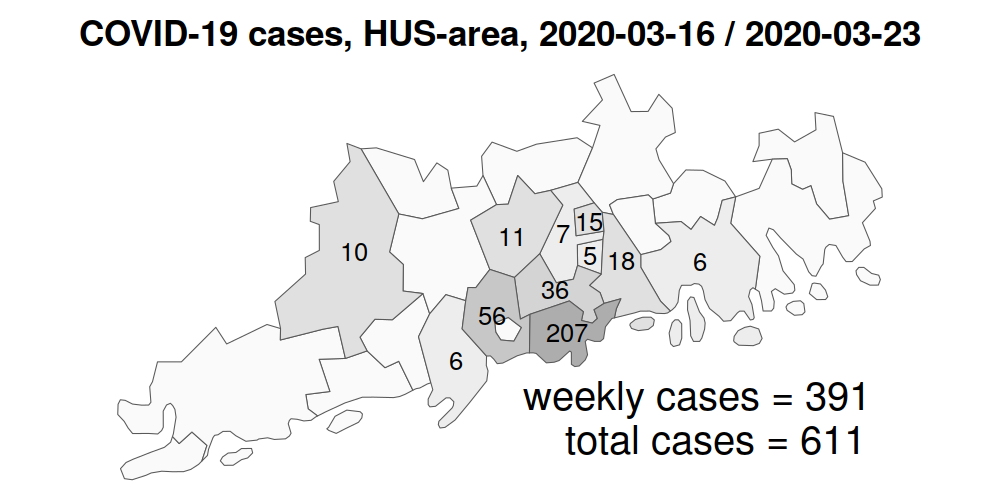
\includegraphics[width = 2.1in]{img/hus_incidence_06.png} \\
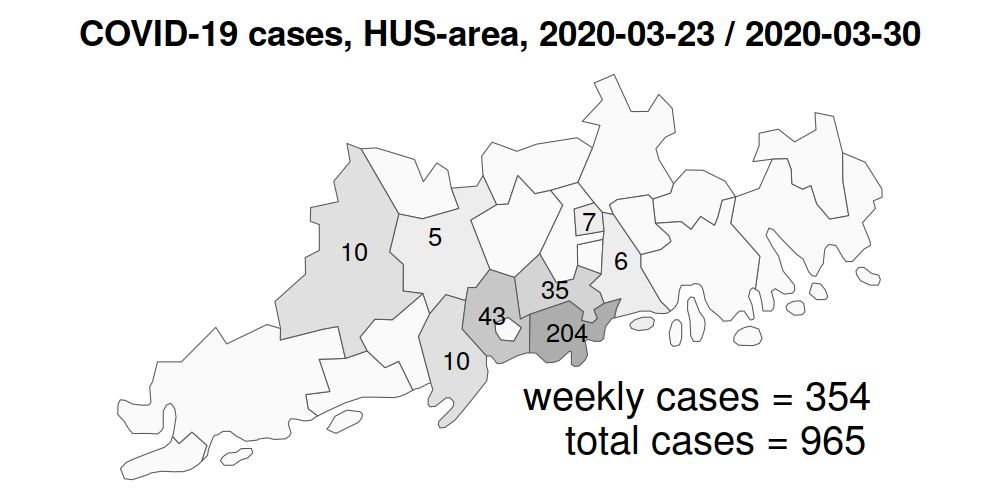
\includegraphics[width = 2.1in]{img/hus_incidence_07.png} &
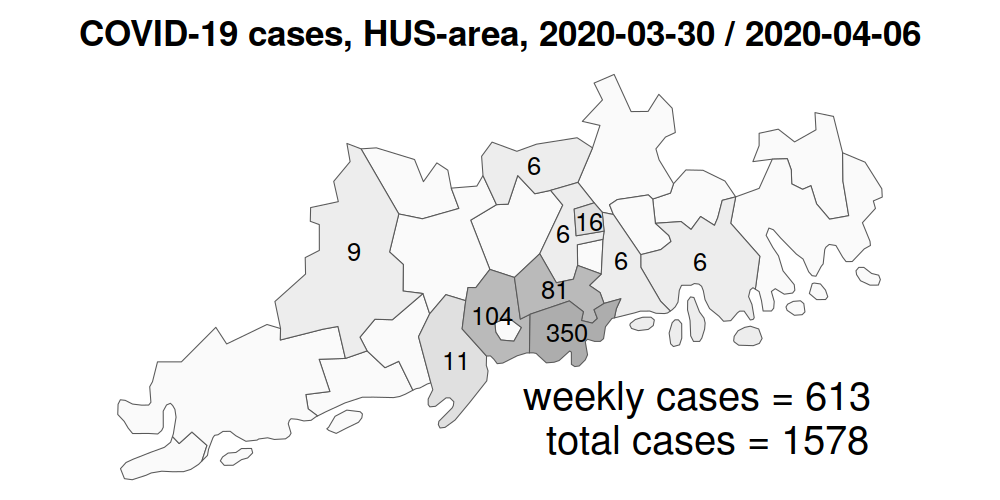
\includegraphics[width = 2.1in]{img/hus_incidence_08.png} &
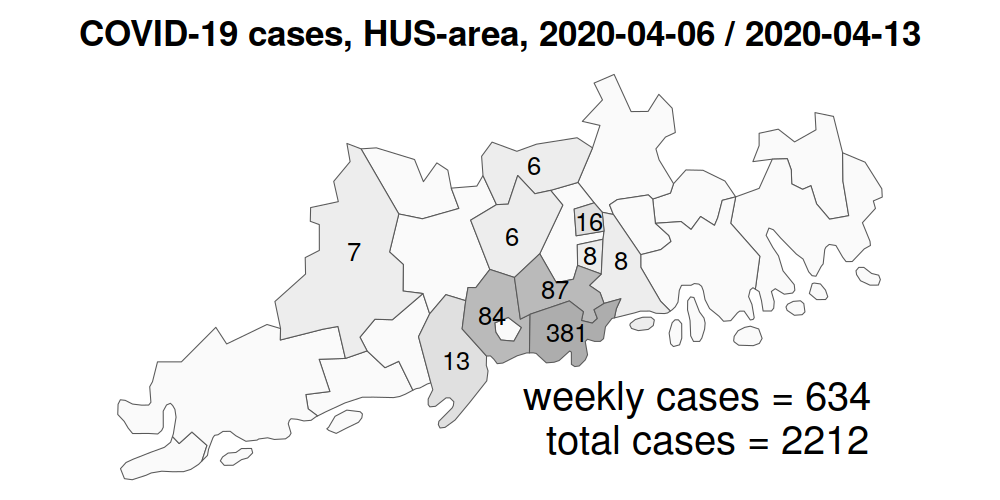
\includegraphics[width = 2.1in]{img/hus_incidence_09.png} \\
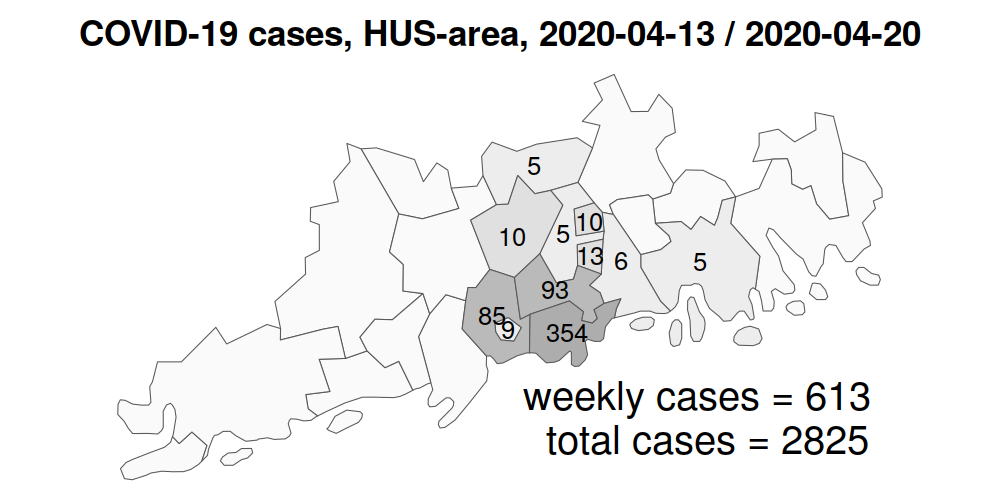
\includegraphics[width = 2.1in]{img/hus_incidence_10.png} &
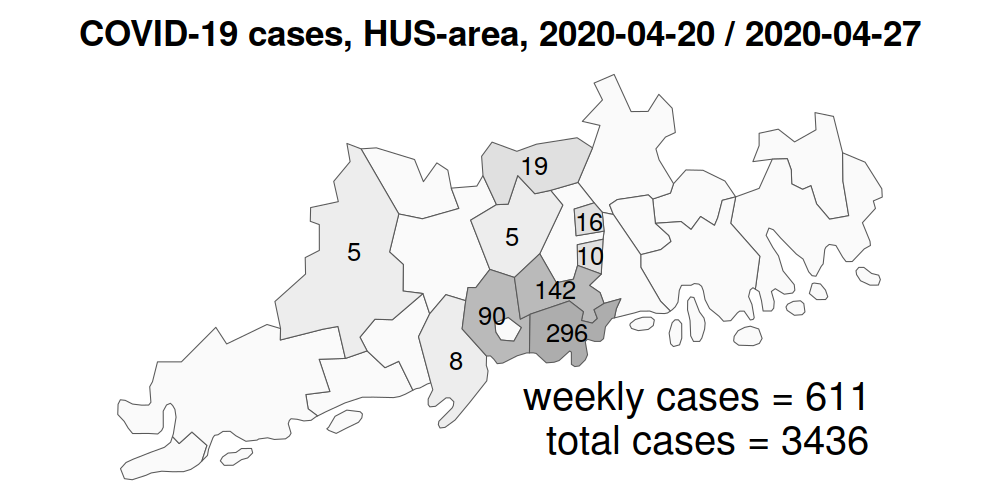
\includegraphics[width = 2.1in]{img/hus_incidence_11.png} &
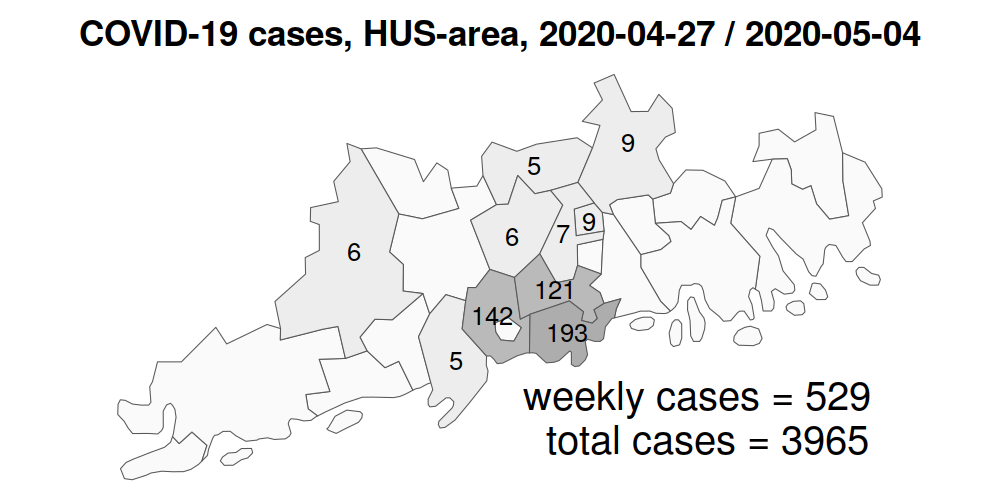
\includegraphics[width = 2.1in]{img/hus_incidence_12.png} \\
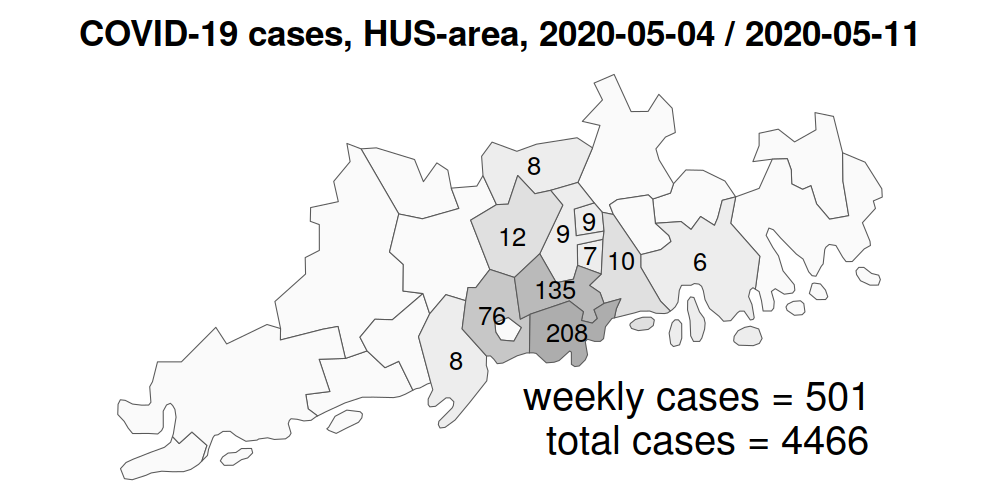
\includegraphics[width = 2.1in]{img/hus_incidence_13.png} &
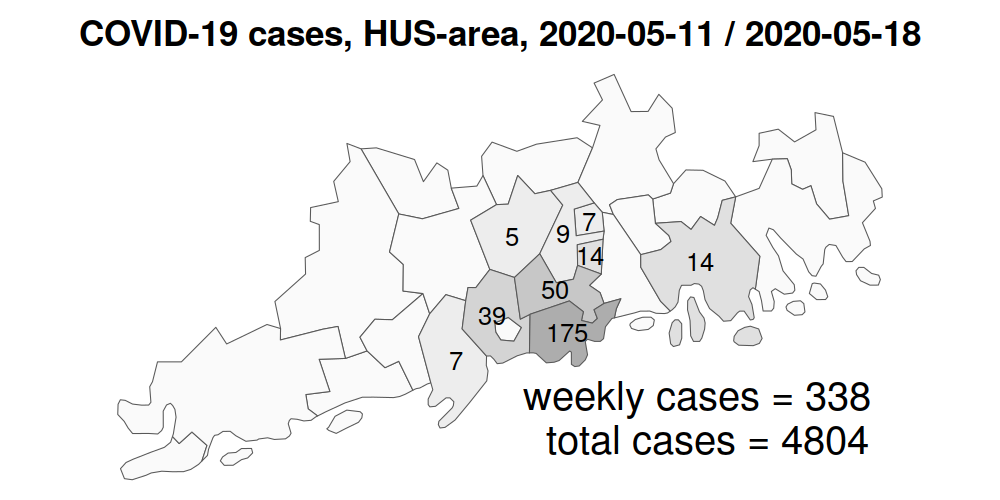
\includegraphics[width = 2.1in]{img/hus_incidence_14.png} &
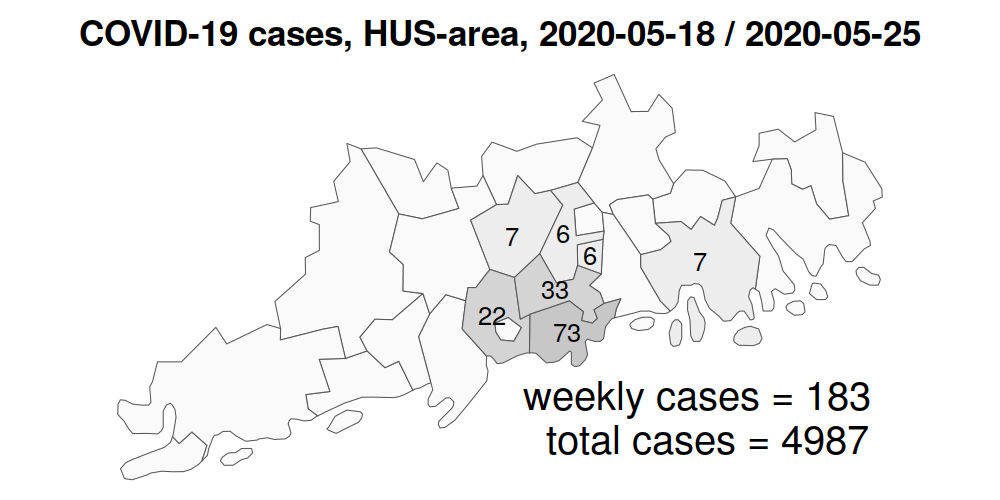
\includegraphics[width = 2.1in]{img/hus_incidence_15.png} \\
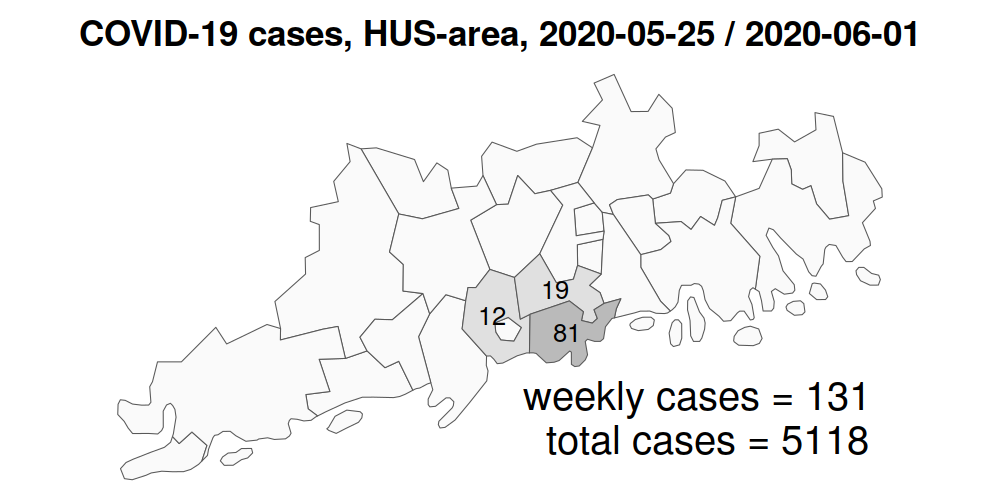
\includegraphics[width = 2.1in]{img/hus_incidence_16.png} &
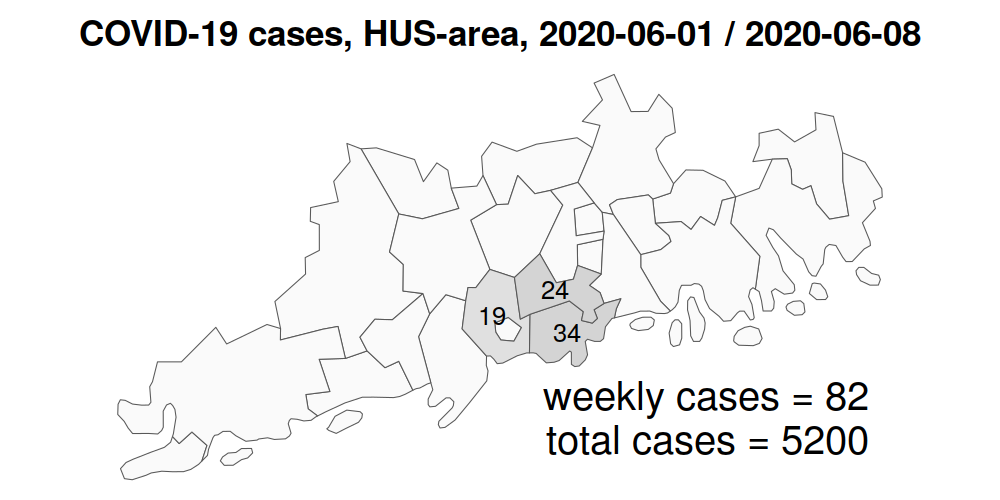
\includegraphics[width = 2.1in]{img/hus_incidence_17.png} &
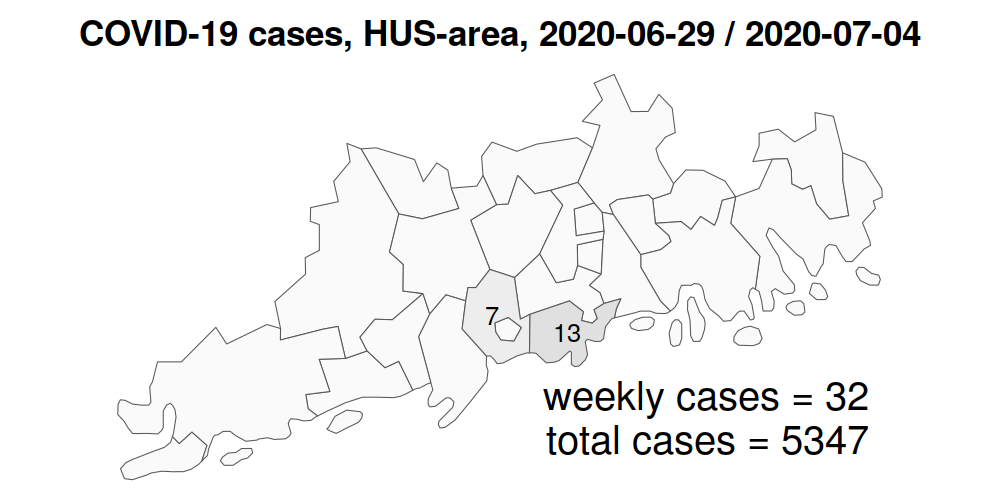
\includegraphics[width = 2.1in]{img/hus_incidence_21.png} 
\end{tabular}

\caption{Numbers of COVID-19 cases by week and municipality in the extended capital region of Helsinki and Uusimaa, Finland (HUS area) during the first wave of the 2020 COVID-19 outbreak. In each map, the number of cases in each municipality is shown if it is 5 or more. Detailed data for three weeks in June (2020-06-08 / 2020-06-15, 2020-06-15 / 2020-06-22 and 2020-06-22 / 2020-06-29), with total 147 cases, are not shown in the figure.}

\label{fig:huscases}
\end{figure}

\newpage

\begin{figure}[!htb]
\centering

\begin{tabular}{cccccccccc}
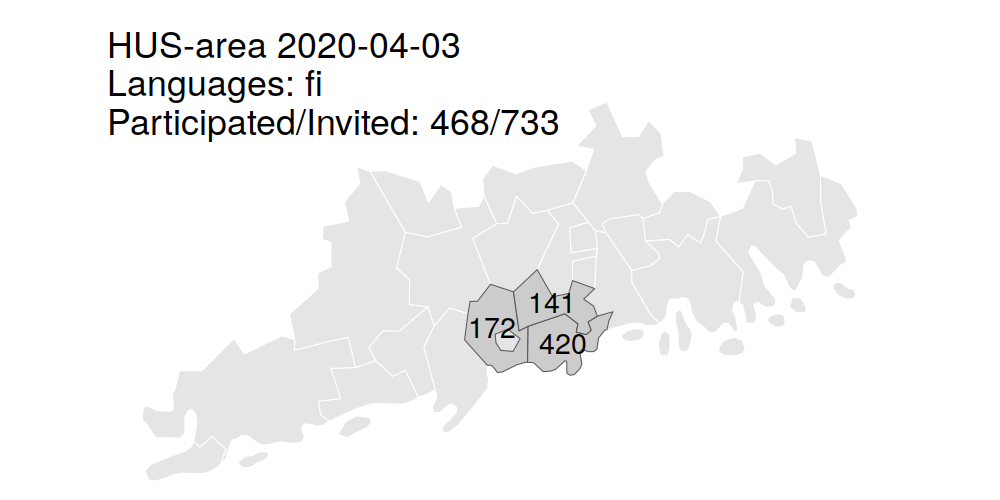
\includegraphics[width = 2.1in]{img/sample01.png} &  
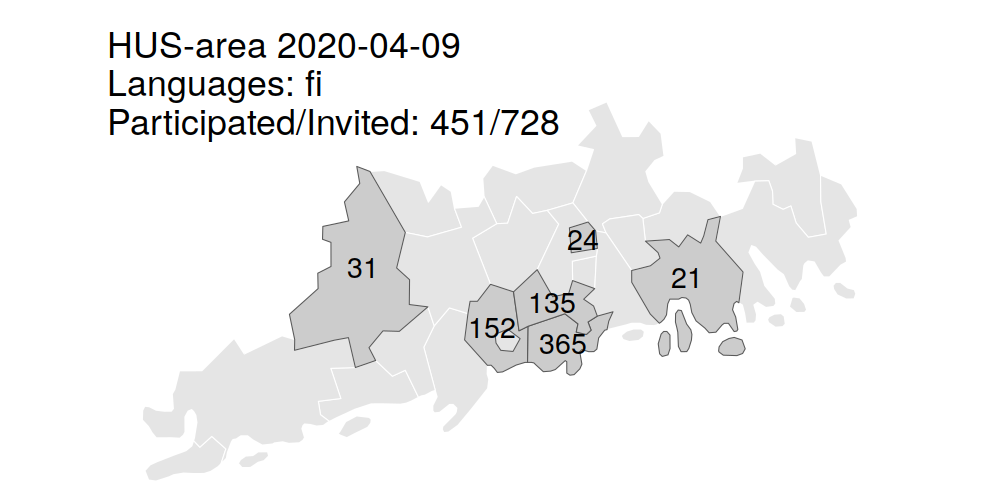
\includegraphics[width = 2.1in]{img/sample02.png} &
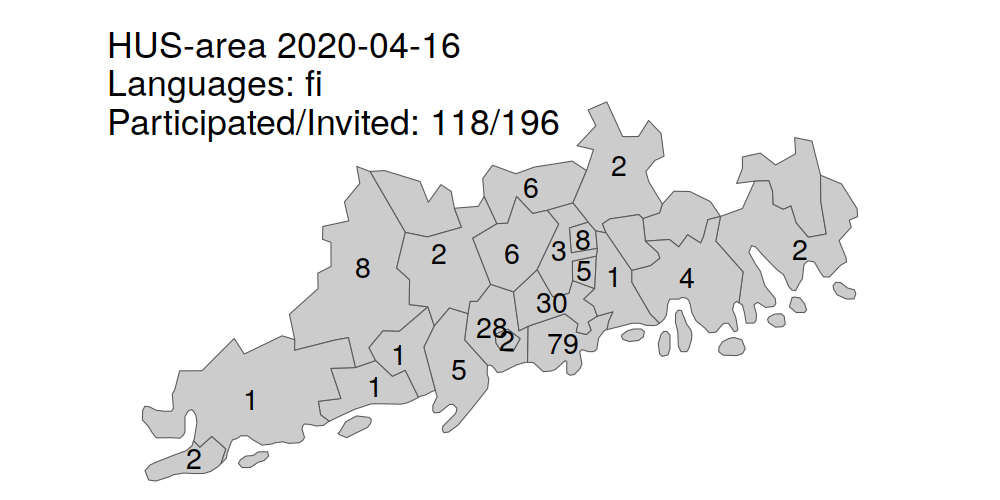
\includegraphics[width = 2.1in]{img/sample03.png} \\
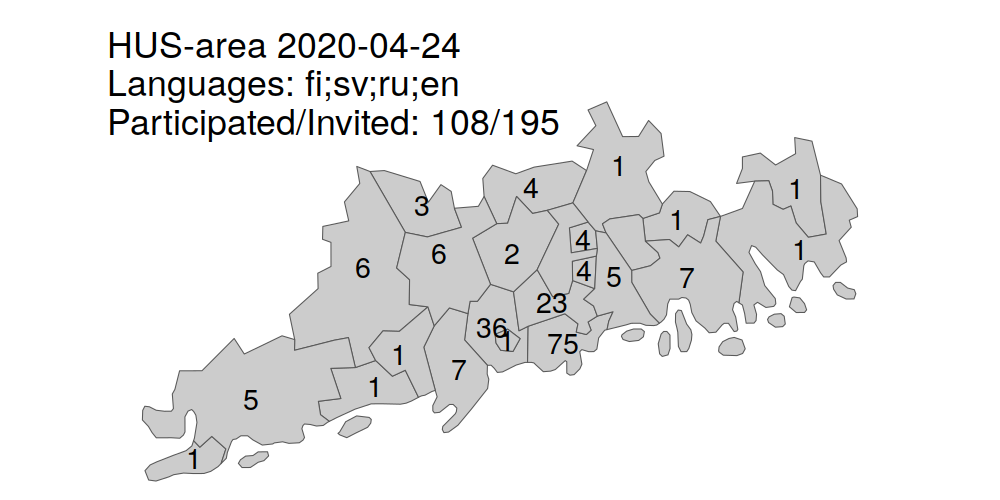
\includegraphics[width = 2.1in]{img/sample04.png} &
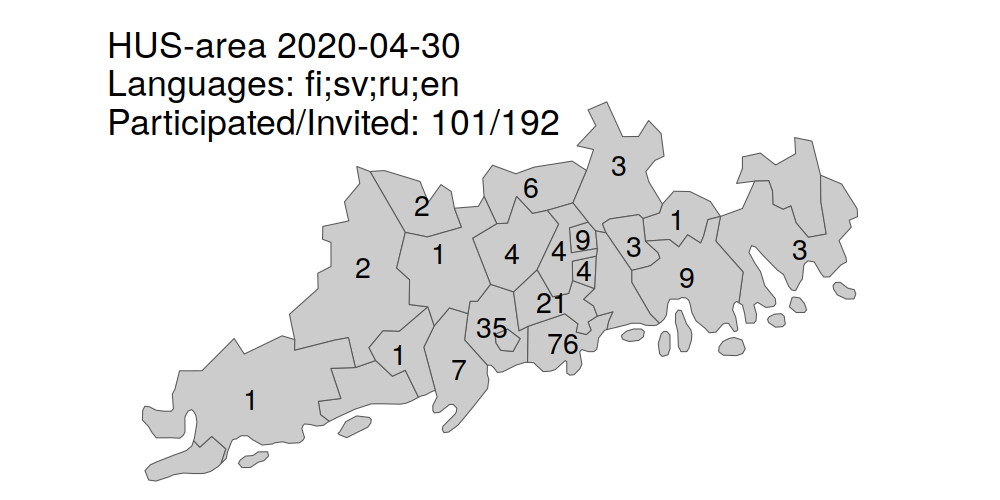
\includegraphics[width = 2.1in]{img/sample05.png} &
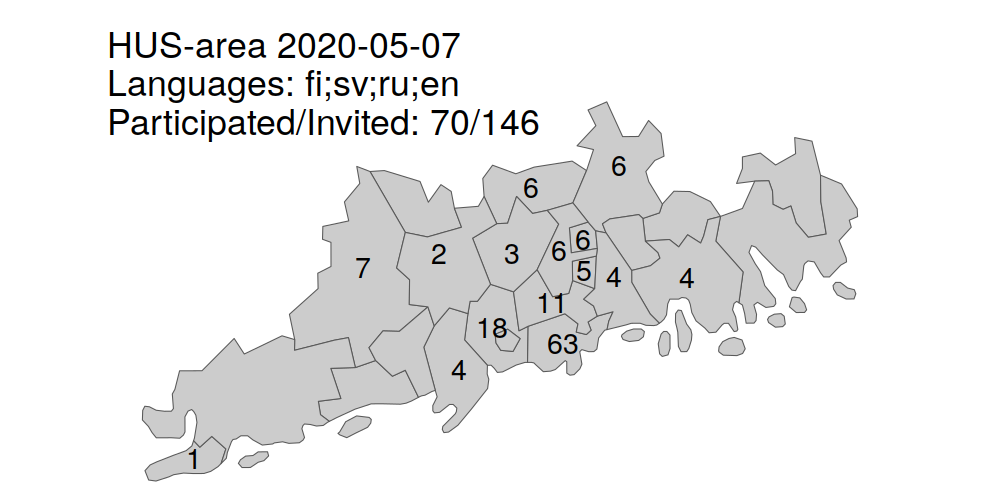
\includegraphics[width = 2.1in]{img/sample06.png} \\
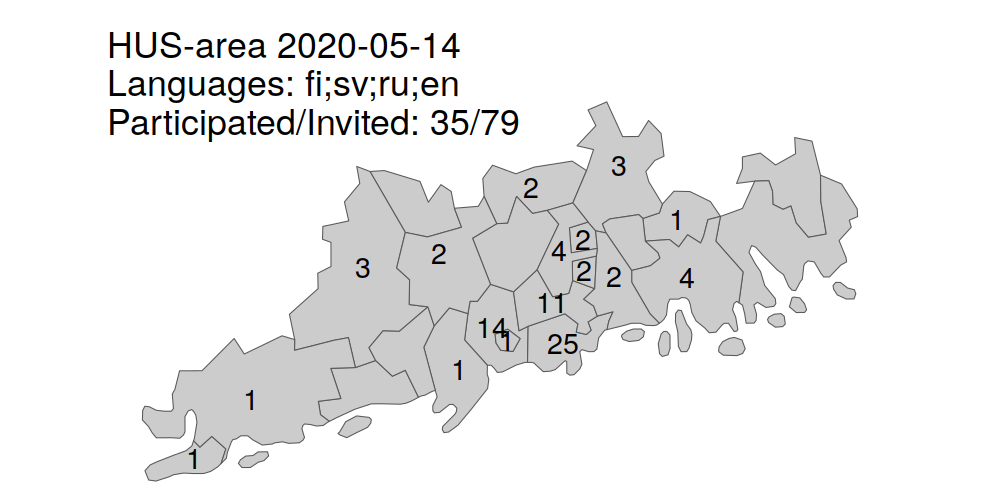
\includegraphics[width = 2.1in]{img/sample07.png} &
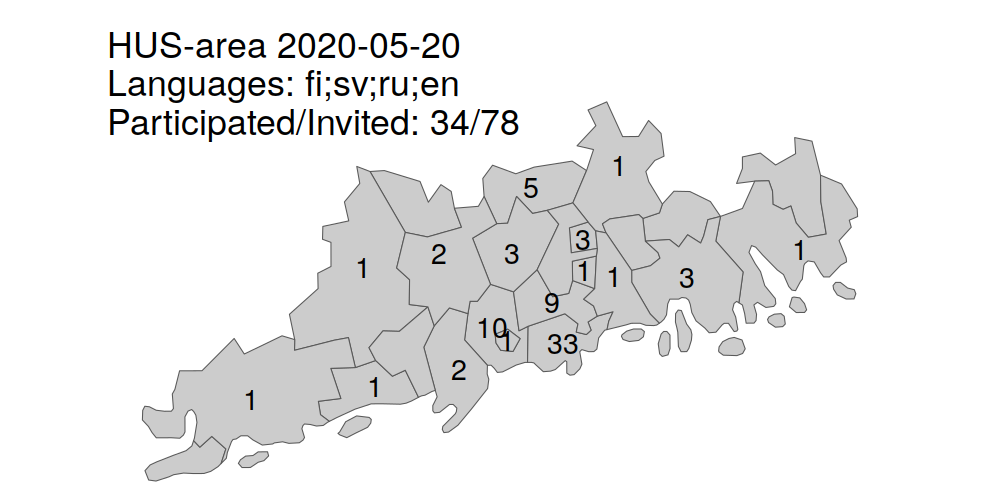
\includegraphics[width = 2.1in]{img/sample08.png} &
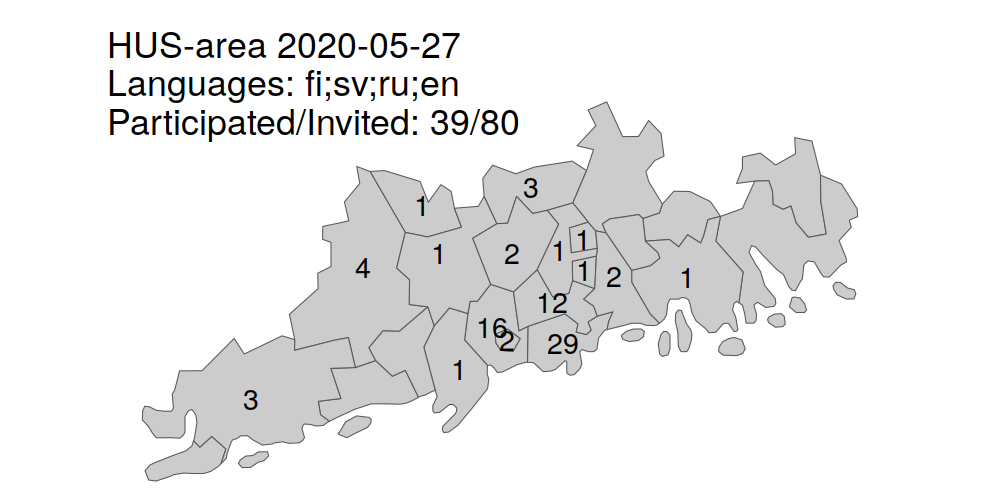
\includegraphics[width = 2.1in]{img/sample09.png} \\
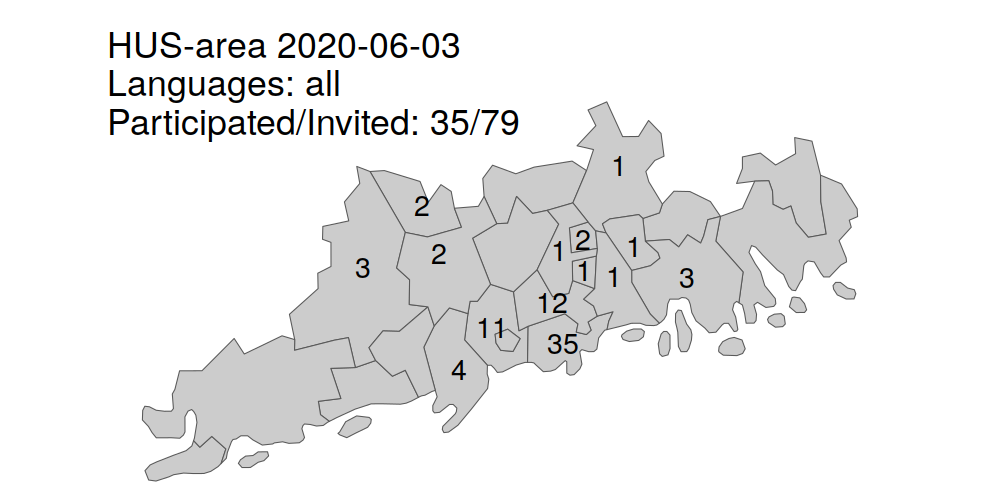
\includegraphics[width = 2.1in]{img/sample10.png} 
\end{tabular}

\caption{Population sampling in the extended capital region of Helsinki and Uusimaa, Finland (HUS area) during the first 10 weeks of the serological surveys. Population sampling was carried out weekly or biweekly and each map corresponds to a single sampling week. The first day of the week and the targeted native languages are listed for each sampling week (fi = Finnish, sv = Swedish, ru = Russian, en = English). The number of invited individuals by municipality are shown on each map. }

\label{fig:survey}
\end{figure}

\newpage

\begin{figure}[!htb]
\centering
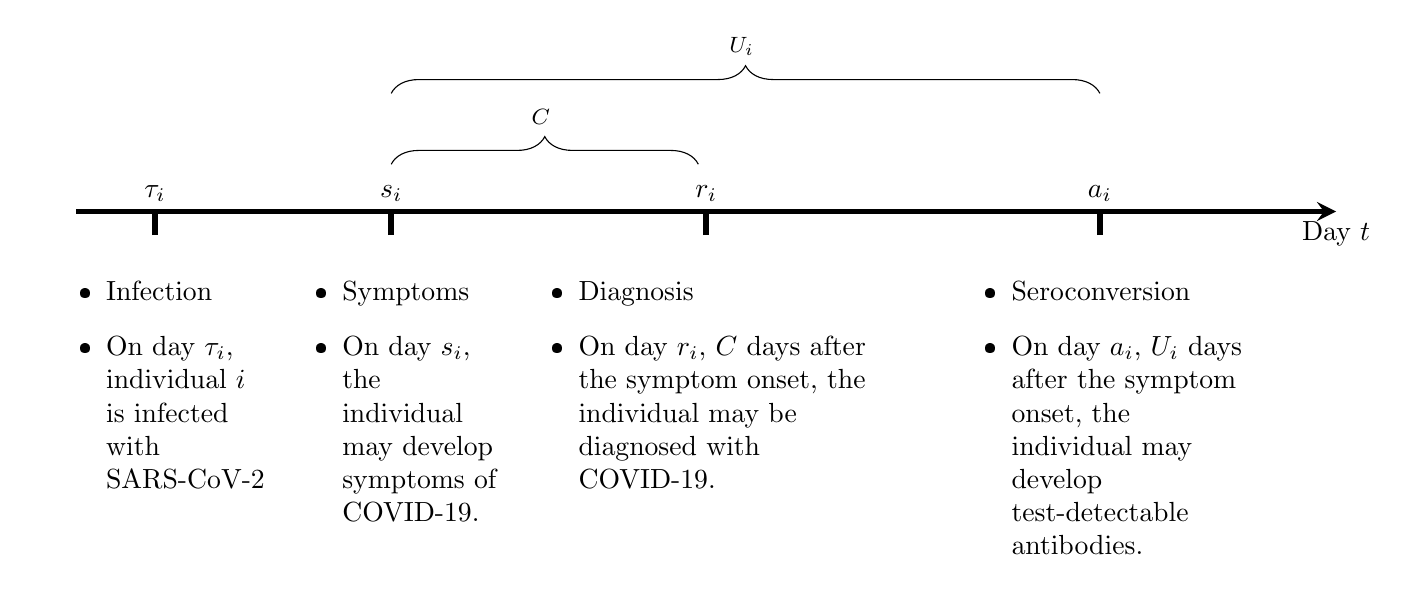
\begin{tikzpicture}
\usetikzlibrary{calc}

% draw arrow
\coordinate (start) at (-1,0);
\coordinate (end) at (15,0);
\draw [line width=2pt, -stealth] (start) -- (end);

% You can use `foreach` to improve the following codes
\coordinate (s0) at (0,-0.3);
\coordinate (t0) at ($(s0)+(0,0.3)$);
\coordinate (s1) at (3,-0.3);
\coordinate (t1) at ($(s1)+(0,0.3)$);
\coordinate (s2) at (7,-0.3);
\coordinate (t2) at ($(s2)+(0,0.3)$);
\coordinate (s3) at (12,-0.3);
\coordinate (t3) at ($(s3)+(0,0.3)$);

\node [anchor=north] at (end.south) {\text{Day} $t$};

% draw ticks
\draw [line width=2pt] (s0) -- (t0);
\node [anchor=south] at (t0.north) {$\tau_i$};

\draw [line width=2pt] (s1) -- (t1);
\node [anchor=south] at (t1.north) {$s_i$};

\draw [line width=2pt] (s2) -- (t2);
\node [anchor=south] at (t2.north) {$r_i$};

\draw [line width=2pt] (s3) -- (t3);
\node [anchor=south] at (t3.north) {$a_i$};

% draw decorations

\draw [decorate,decoration={brace,amplitude=10pt},xshift=-3pt,yshift=0pt]
($(t1)+(0, 0.6)$) -- ($(t2)+(-0.1,0.6)$) node [black,midway,xshift=-0.05cm,yshift=0.6cm] 
{\footnotesize $C$};

\draw [decorate,decoration={brace,amplitude=10pt},xshift=-3pt,yshift=0pt]
($(t1)+(0, 1.5)$) -- ($(t3)+(0,1.5)$) node [black,midway,xshift=-0.05cm,yshift=0.6cm] 
{\footnotesize $U_i$};


% add texts
\node [anchor=north, align=left, text width=3cm] at (s0.south) {
\begin{itemize}
\item Infection 
\item On day $\tau_i$, individual $i$ is infected with SARS-CoV-2
\end{itemize}
};

\node [anchor=north, align=left, text width=3cm] at (s1.south) {
\begin{itemize}
\item Symptoms
\item On day $s_i$, the individual may develop symptoms of COVID-19.
\end{itemize}
};

\node [anchor=north, align=left, text width=5cm] at (s2.south) {
\begin{itemize}
\item Diagnosis
\item On day $r_i$, $C$ days after the symptom onset, the individual may be diagnosed with COVID-19.
\end{itemize}
};

\node [anchor=north, align=left, text width=4cm] at (s3.south) {
\begin{itemize}
\item Seroconversion
\item On day $a_i$, $U_i$ days after the symptom onset, the individual may develop test-detectable antibodies.
\end{itemize}
};

\end{tikzpicture}

\caption{Timeline from a SARS-CoV-2 infection to seroconversion.} 
\label{fig:seroconv}
\end{figure}

\newpage


\begin{figure}[!htb]

% https://github.com/xinychen/awesome-latex-drawing
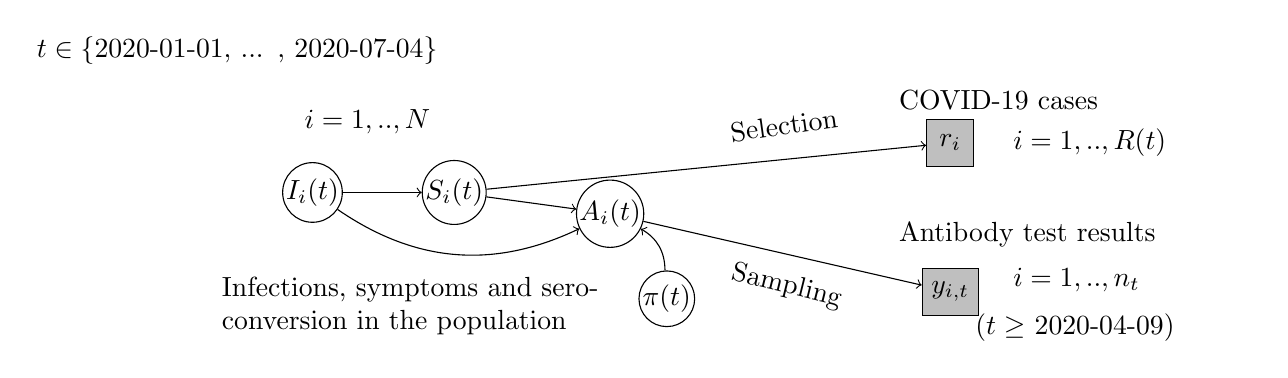
\begin{tikzpicture}[
    scale = 0.9,
    param/.style={shape=circle, draw=black,fill=white,inner sep=0pt,minimum size=0.6cm},
    obs/.style={shape=rectangle, draw=black, fill=lightgray, minimum size=0.6cm}
  ]
  
    % time t
    \node [text width=7cm] (T) at (-3.0, 1)  {$t \in \{$\printdate{2020-01-01}, ... , \printdate{2020-07-04}$\}$};
    
    % infections
    \node [param] (inf) at (-3,-1) {$I_i(t)$};
    
    % symptoms
    \node [param] (symp) at (-1,-1) {$S_i(t)$};    
    
    % antibodies
    \node [param] (sero) at (1.2,-1.3) {$A_{i}(t)$};
    
    % seroprevalence
    \node [param] (prevalence) at (2, -2.5) {$\pi(t)$};
    
    
    % text for population plate
    \node [text width=5cm] (latent) at (-1.5,-2.6)  {Infections, symptoms and seroconversion in the population};
    
    % label and plate for population
    \node [text width=2cm] (N) at (-2, 0)  {$i = 1, .., N$};
    \plate[]{POP}{(inf)(sero)(N)(latent)(prevalence)}{};

    
    % registered disease cases
    % ---
    
    % Selection
    \node [text width=2cm, rotate=8] (ttrsampling) at (4,0) {Selection};
    
    % r_i
    \node [obs]  (ttr) at (6,-0.3) {$r_i$}; 
    
    % label
    \node [text width=4cm] (registry) at (7.5,0.3) {COVID-19 cases};
    
    % R(t)
    \node [text width=2cm] (nobs) at (8,-0.3)   {$i = 1, .., R(t)$};  
    

    
    % Antibody test results 
    % ---
    
    % Sampling
    \node [text width=2cm, rotate=-14] (serosampling) at (4, -1.5*1.6) {Sampling};    
    
    %  y
    \node [obs]  (y) at (6,-1.5*1.6) {$y_{i, t}$};   
    
    % label
    \node [text width=4cm] (serosurvey) at (7.5,-1.6)  {Antibody test results};

    % n_t
    \node [text width=2cm] (nsero) at (8,-1.6*1.4)  {$i = 1, .., n_{t}$};  
    
    % t sero
    \node [text width=3.5cm] (serosurvey_t) at (8.3,-2.9)  {($t \geq$ \printdate{2020-04-09})};


    
    % paths
    \path [draw,->] (inf) edge (symp);
    \path [draw,->] (inf) edge [bend right] (sero);
    \path [draw,->] (symp) edge (sero);
    \path [draw,->] (sero) edge (y);
    \path [draw,->] (symp) edge (ttr);
    
    \path [draw,->] (prevalence) edge [bend right] (sero);

    % plate for antibody observations
    \plate[]{SERO}{(y)(serosurvey)(nsero)}{}
    
    % plate for infection observations
    \plate[]{TTR}{(ttr)(registry)(nobs)}{}
    
    
    \plate[]{TIME}{(T)(POP)(TTR)(SERO)}{}
    
    \plate[white]{ALL}{(TIME)}{}
    
 
    
\end{tikzpicture}
\caption{SARS-CoV-2 infections are observed as diagnosed COVID-19 disease cases or by antibody testing in the participants of the serological surveys. Here, $I_i(t)$ indicates SARS-CoV-2 infection in individual $i$ by day $t$; $S_i(t)$ indicates symptom onset in individual $i$ by day $t$; $r_i$ is the diagnosis day of a COVID-19 case, with a total $R(t)$ cases by day $t$; $A_i(t)$ indicates seroconversion in individual $i$ by day $t$, possibly observed as a positive antibody test $y_{i, t} = 1$ among $n_t$ blood samples taken on day $t$; $\pi(t)$ indicates the proportion of seroconverted individuals in the population of size $N$ (seroprevalence).} 
\label{fig:models}

\end{figure} 

\newpage

\begin{figure}[!htb]

% https://github.com/xinychen/awesome-latex-drawing
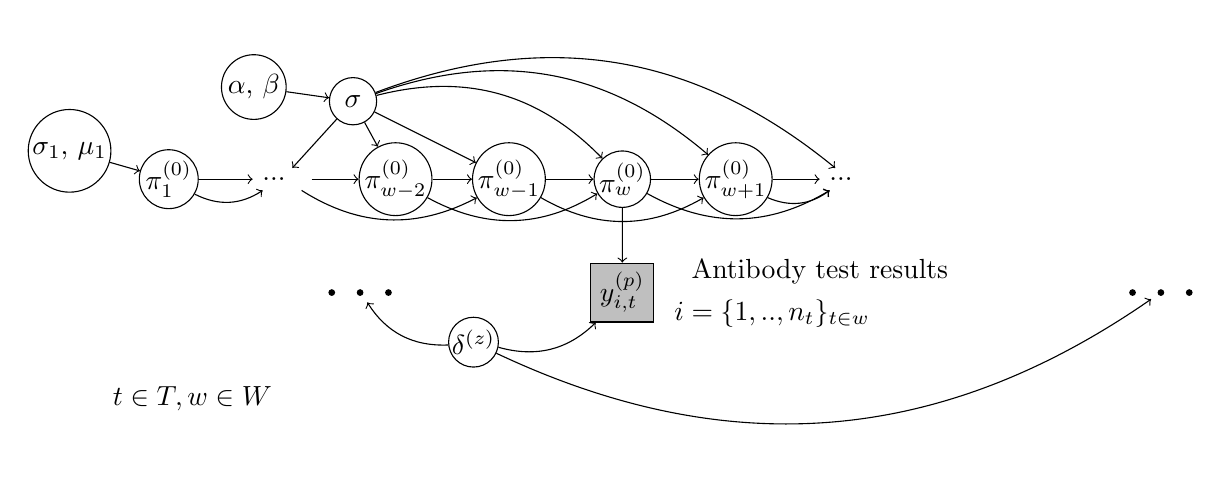
\begin{tikzpicture}[scale=0.9]
    
    % antibody prevalence

    % prior for w 0
    \node [circle,draw=black,fill=white,inner sep=0pt,minimum size=0.6cm] (serow1) at (-1.6,1.6) {$\pi^{(0)}_{1}$};
    
    % ...
    \node [text width=0.5cm] (serodot1) at (0,1.6) {...};  
    
    % w - 2
    \node [circle,draw=black,fill=white,inner sep=0pt,minimum size=0.6cm] (serow-2) at (1.6, 1.6) {$\pi^{(0)}_{w-2}$};
    
    % w - 1
    \node [circle,draw=black,fill=white,inner sep=0pt,minimum size=0.6cm] (serow-1) at (2*1.6, 1.6) {$\pi^{(0)}_{w-1}$};   
    
    % w
    \node [circle,draw=black,fill=white,inner sep=0pt,minimum size=0.6cm] (serow) at (3*1.6, 1.6) {$\pi^{(0)}_{w}$};
    
    % w + 1 ...
    \node [circle,draw=black,fill=white,inner sep=0pt,minimum size=0.6cm] (serow+1) at (4*1.6, 1.6) {$\pi^{(0)}_{w+1}$};
    \node [text width=0.5cm] (serodot2) at (5*1.6,1.6) {...};  
    
    
    % mu 1, sigma 1
    \node [circle,draw=black,fill=white,inner sep=1pt,minimum size=0.6cm] (sigma1) at (-3, 2) {$\sigma_1$, $\mu_1$};
    
    % sigma    
    \node [circle,draw=black,fill=white,inner sep=0pt,minimum size=0.6cm] (sigma) at (1, 2.7) {$\sigma$};
    
    % alpha and beta for sigma
    \node [circle,draw=black,fill=white,inner sep=1pt,minimum size=0.7cm] (ab) at (-0.4, 2.9) {$\alpha$, $\beta$};
   
    \path [draw,->] (ab) edge (sigma); 

    
    % dependencies s -> s direct
     \path [draw,->] (serow1) edge (serodot1);   
     \path [draw,->] (serodot1) edge (serow-2);   
     \path [draw,->] (serow-2) edge (serow-1);   
     \path [draw,->] (serow-1) edge (serow);   
     \path [draw,->] (serow) edge (serow+1);   
     \path [draw,->] (serow+1) edge (serodot2);   
     
    % dependencies s -> s indirect
     \path [draw,->] (serow1) edge [bend right] (serodot1);   
     \path [draw,->] (serodot1) edge [bend right] (serow-1);   
     \path [draw,->] (serow-2) edge [bend right] (serow);   
     \path [draw,->] (serow-1) edge [bend right] (serow+1);   
     \path [draw,->] (serow) edge [bend right] (serodot2);  
     \path [draw,->] (serow+1) edge [bend right] (serodot2);   

 
    % paths for sigma
    \path [draw,->] (sigma) edge (serodot1); 
   \path [draw,->] (sigma1) edge (serow1);   
   \path [draw,->] (sigma) edge (serow-2);   
   \path [draw,->] (sigma) edge (serow-1);   
   \path [draw,->] (sigma) edge [bend left] (serow);   
   \path [draw,->] (sigma) edge [bend left] (serow+1);   
   \path [draw,->] (sigma) edge [bend left] (serodot2); 
  
    
    % Antibody test results
    \node [text width=4cm] (obslabel) at (5*1.6,0.3)  {Antibody test results};  
    
    \node [rectangle,draw=black,fill=lightgray] (yw) at (3*1.6,0) {$y^{(p)}_{i, t}$};  
    
    \node [text width=3cm] (nsero) at (4.5*1.6,-0.3)  {$i = \{1, .., n_{t} \}_{t \in w}$}; 
    
    \plate[] {YW}{(yw)(nsero)(obslabel)}{}

    % dots for obs, left of y
    \node[mark size=1pt,color=black] (ydot1) at (0.7,0) {\pgfuseplotmark{*}};
    \node[mark size=1pt,color=black] (serodotleft) at (0.7+0.4,0) {\pgfuseplotmark{*}};
    \node[mark size=1pt,color=black] at (0.7+0.8,0) {\pgfuseplotmark{*}};
    
    % dots for obs, right of y
    \node[mark size=1pt,color=black] at (7.5*1.6,0) {\pgfuseplotmark{*}};
    \node[mark size=1pt,color=black] (serodotright) at (7.5*1.6+0.4,0) {\pgfuseplotmark{*}};
    \node[mark size=1pt,color=black] (ydot2) at (7.5*1.6+0.8,0) {\pgfuseplotmark{*}};
    
    
    % test specificity
    \node [circle,draw=black,fill=white,inner sep=0pt,minimum size=0.6cm] (spec) at (2.7,-0.7) {$\delta^{(z)}$};

    
   \path [draw,->] (serow) edge (yw);   
   \path [draw,->] (spec) edge [bend right] (yw);   
   \path [draw,->] (spec) edge [bend left] (serodotleft);   
   \path [draw,->] (spec) edge [bend right] (serodotright); 
   

    % study period
    \node [text width=2.5cm] (t) at (-1,-1.5) {$t \in T, w \in W$}; 
    
    % plate for all
    \plate[]{T}{(YW)(spec)(sigma1)(ab)(ydot1)(ydot2)(t)}{}

 
    
\end{tikzpicture}

\caption{The model for seroprevalence $\pi^{(0)}(t)$ (Estimation model). The study period $T$ is split into weeks $W$. On day $t$ during the study period, where $t$ belongs to week $w$, the antibody test result $y^{(z)}_{i, t}$ for individual $i$, $i = {1, ..., n_t}_{t \in w}$, depends on the seroprevalence $\pi^{(0)}_w$ during week $w$ and the specificity $\delta^{(z)}$ of the antibody test $z$, where $z \in \{\text{Screen}, \text{Confirmation}\}$. In the prior distribution, the seroprevalence during the first week $\pi_1^{(0)}$is distributed according to parameters $\mu_1$ and $\sigma_1^2$, and the seroprevalence during week $w$ depends on the two previous weeks. The strength of the dependency is controlled by $\sigma$, with a prior distribution depending on parameters $\alpha$ and $\beta$. } 
\label{fig:model1}

\end{figure}

\newpage

\begin{figure}[!htb]

% https://github.com/xinychen/awesome-latex-drawing
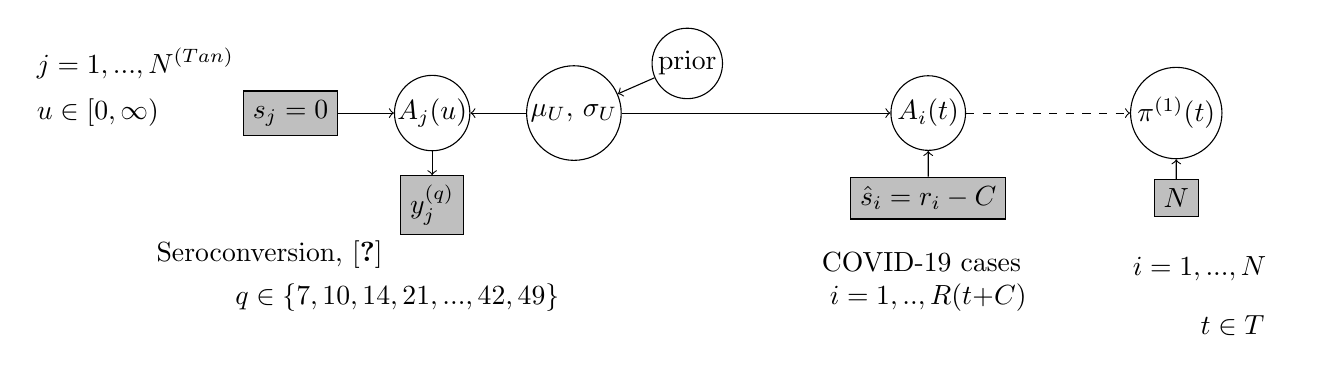
\begin{tikzpicture}[scale=0.9]
    
    % Tan model
    
    % N
    \node [text width=5cm] (TanN) at (-2.8, 2.7)  {$j = 1, ..., N^{(Tan)}$};    
    
    % d
    \node [text width=5cm] (Ttan) at (-2.8, 2)   {$u  \in [0, \infty)$};

    % S
    \node [rectangle,draw=black,fill=lightgray] (S) at (-2, 2) {$s_j = 0$};  
    
    % A
    \node [circle,draw=black,fill=white,inner sep=0pt,minimum size=0.6cm] (Atan) at (0, 2) {$A_j(u)$};
    
    % mu U , sigma U
    \node [circle,draw=black,fill=white,inner sep=1pt,minimum size=0.5cm] (musigma) at (2, 2) {$\mu_U$, $\sigma_U$};
  
    % prior 
    \node [circle,draw=black,fill=white,inner sep=1pt,minimum size=0.5cm] (musigmaprior) at (3.6, 2.7) {prior};   
    
     % Seroconversion
    
    % y
    \node [rectangle,draw=black,fill=lightgray] (y) at (0, 0.7) {$y_j^{(q)}$};  
    
    % label
    \node [text width=7cm] (tanlabel) at (0, 0)  {Seroconversion, \cite{Tan2020}}; 
    
    % Q
    \node [text width=5cm] (Qtan) at (0, -0.6)  {$q  \in \{7, 10, 14, 21, ..., 42, 49\}$};

    \plate[] {Y}{(y)(tanlabel)(Qtan)}{}
    
    \plate[] {TAN}{(TanN)(Y)(Atan)(musigma)(musigmaprior)}{}
    


    \path [draw,->] (Atan) edge (y);   
    \path [draw,->] (S) edge (Atan);   
    \path [draw,->] (musigma) edge (Atan); 
    
    
    % FNIDR projection
    % ---

    % projected A_i(t)
    \node [circle,draw=black,fill=white,inner sep=1pt,minimum size=0.6cm] (Ahus) at (7, 2) {$A_i(t)$};
    
    % Registered disease cases
    % ----
    
    % r_i
    \node [rectangle,draw=black,fill=lightgray] (r) at (7, 0.8) {$\hat{s}_i = r_{i} - C$}; 
    
    % label
    \node [text width=2.7cm] (obslabel) at (7, -0.1)  {COVID-19 cases}; 
    
    % i = 1, .., R(t)
    \node [text width=2.5cm] (nobs) at (7, -0.6)  {$i = 1, .., R(t + C)$}; 
    
    % plate
    \plate[] {TTR}{(r)(nobs)(obslabel)}{}   

    
    % prevalence
    \node [circle,draw=black,fill=white,inner sep=1pt,minimum size=0.6cm] (pi) at (10.5, 2) {$\pi^{(1)}(t)$};
    
    \node [rectangle,draw=black,fill=lightgray] (N) at (10.5, 0.8) {$N$}; 
    
    % HUS N
    \node [text width=2cm] (NHUS) at (11.0, -0.2)  {$i = 1, ..., N$};    

    % HUS time
    \node [text width=1cm] (T) at (11.4, -1)  {$t  \in T$};

    
    \plate[] {HUS}{(NHUS)(TTR)(Ahus)(pi)(T)}{}   
    \plate[white]{ALL}{(HUS)(TAN)}{}

    
    \path [draw,->] (musigmaprior) edge (musigma); 
        
    \path [draw,->] (musigma) edge (Ahus); 

    \path [draw,->] (r) edge (Ahus); 
    \path [draw,->, dashed] (Ahus) edge (pi); 
    \path [draw,->] (N) edge (pi); 

    
    
    
\end{tikzpicture}

\caption{The model for seroprevalence $\pi^{(1)}(t)$ (Projection model). Left plate: The duration from symptoms to seroconversion was modelled based on data from \cite{Tan2020}. Individuals $j$, $j = 1, .., N^{(Tan)}$, experienced COVID-19 symptoms on day $s_j = 0$ and were tested for antibodies $q$ days later, where $q$ varied from 7 to 49 days. Individuals were tested on multiple days. Here, $A_j(u)$ denotes whether individual $j$ had seroconverted by day $u$, and ($y_j^{(q)}$) indicates the result of an antibody test taken on the $q$:th day. The duration from symptoms to seroconversion was modelled as a lognormal distribution with parameters $(\mu_U, \sigma_U)$. Right plate: The posterior distribution of $(\mu_U, \sigma_U)$ is utilised to project the seroconversion status $A_i(t)$ for each individual $i = 1, ..., R(t + C)$ with COVID-19 symptom onset before day $t \in T$ during the study period. The symptoms are assumed to have occurred on day $\hat{s}_i = r_i - C$, where $C$ is the lag from symptom onset to the COVID-19 diagnosis day $r_i$. The individual projections are used to derive the population level projection for the seroprevalence on day $t$, $\pi^{(1)}(t)$.} 
\label{fig:model2}

\end{figure}


\newpage


\begin{figure}[!htb]
\centering


\begin{subfigure}{0.47\textwidth}
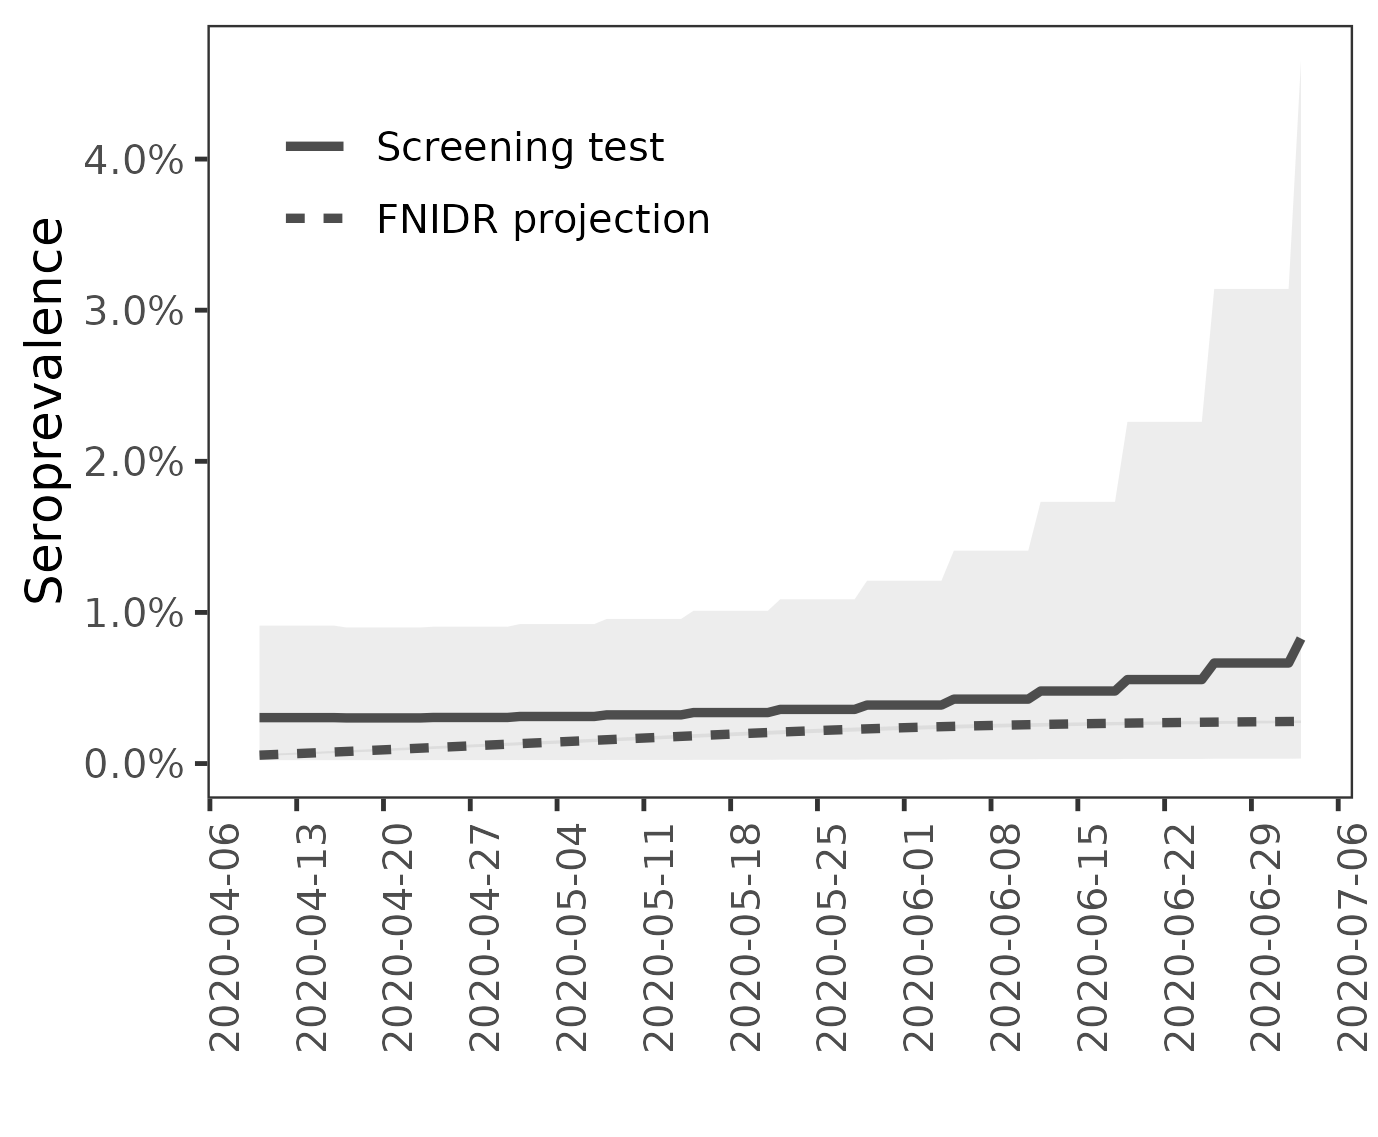
\includegraphics[width=\linewidth]{img/ttr_screen.png}
\caption{Posterior means and 95\% credible intervals of seroprevalence $\pi^{(0)}(t)$ (Screening test) and projected seroprevalence $\pi^{(1)}(t)$}  \label{fig:ttr_screen}
\end{subfigure}%
\hspace*{\fill}
\begin{subfigure}{0.47\textwidth}
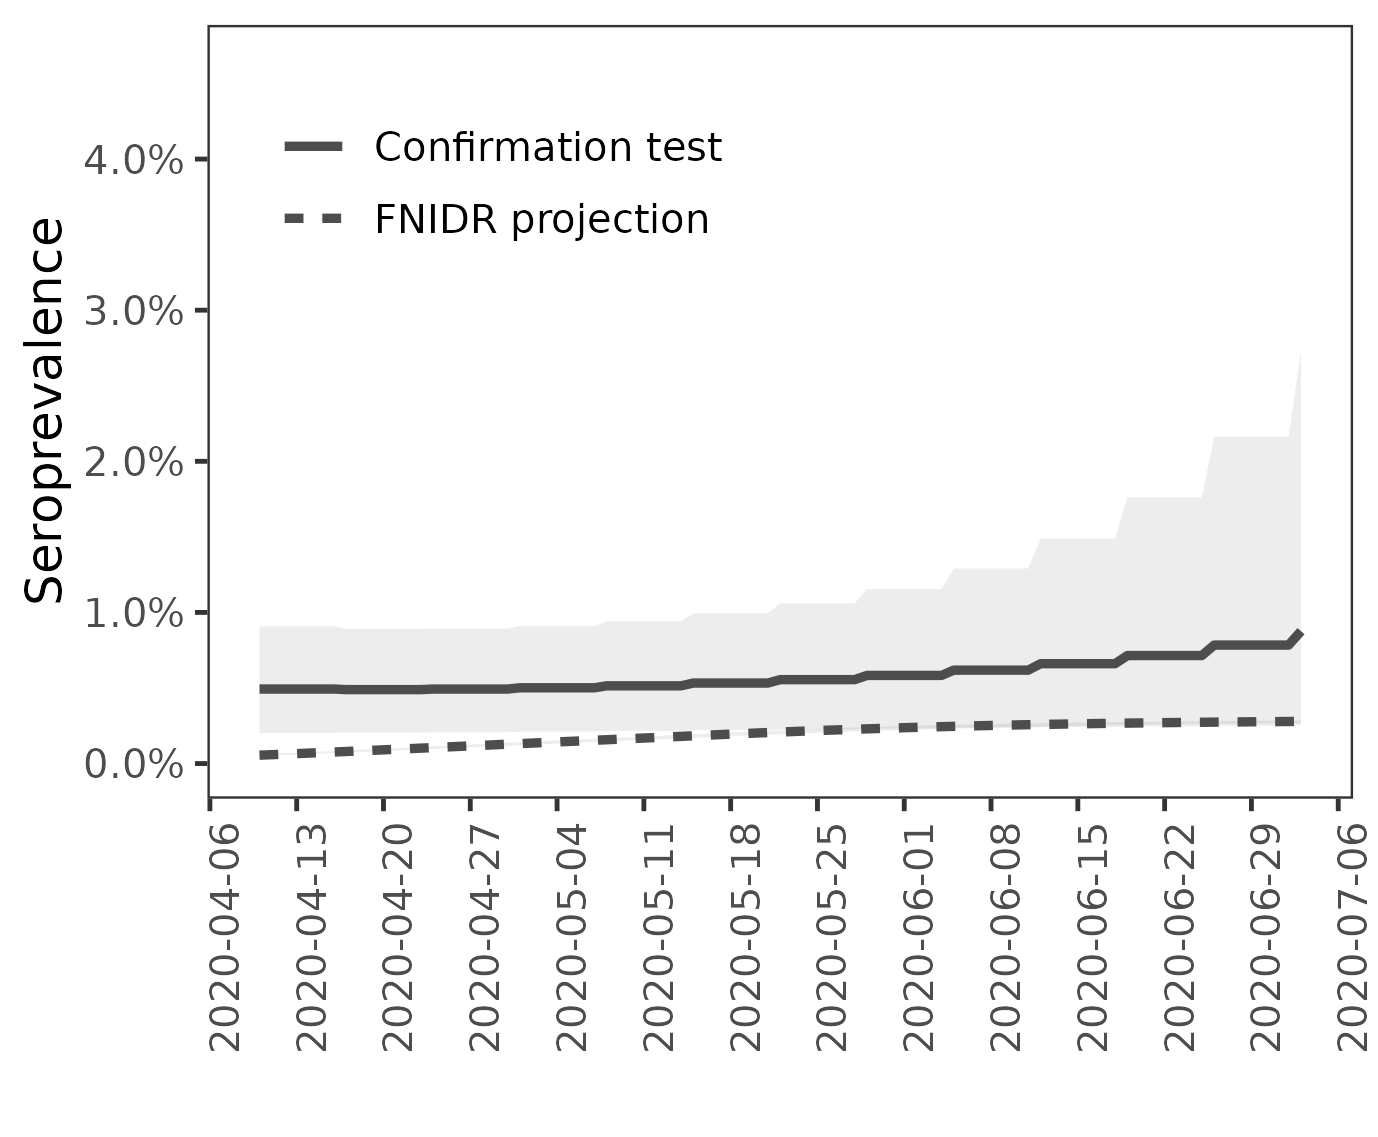
\includegraphics[width=\linewidth]{img/ttr_mnt.png} 
\caption{Posterior means and 95\% credible intervals of seroprevalence $\pi^{(0)}(t)$ (Confirmation test) and projected seroprevalence $\pi^{(1)}(t)$} \label{fig:ttr_mnt}
\end{subfigure}

\caption{Seroprevalence in the extended capital region of Finland during the first wave of the COVID-19 epidemic. Both images show the estimates $\pi^{(0)}(t)$ and projections $\pi^{(1)}(t)$ for seroprevalence using the serology survey observations and COVID-19 cases (FNIDR projection), respectively. The image on the left shows results for the screening test and the image on the right shows results for the confirmation test. Solid lines are posterior means and the shaded areas correspond to 95\% credible intervals derived from the pointwise 2.5\% and 97.5\% quantiles. The dashed lines show the projected seroprevalence and the shaded areas correspond to 95\% credible intervals, however, the intervals for projected seroprevalence are very narrow and not visible.}

\label{fig:seroprevalence}
\end{figure}


\newpage


\begin{figure}[!htb]
\centering

\begin{subfigure}{0.45\textwidth}
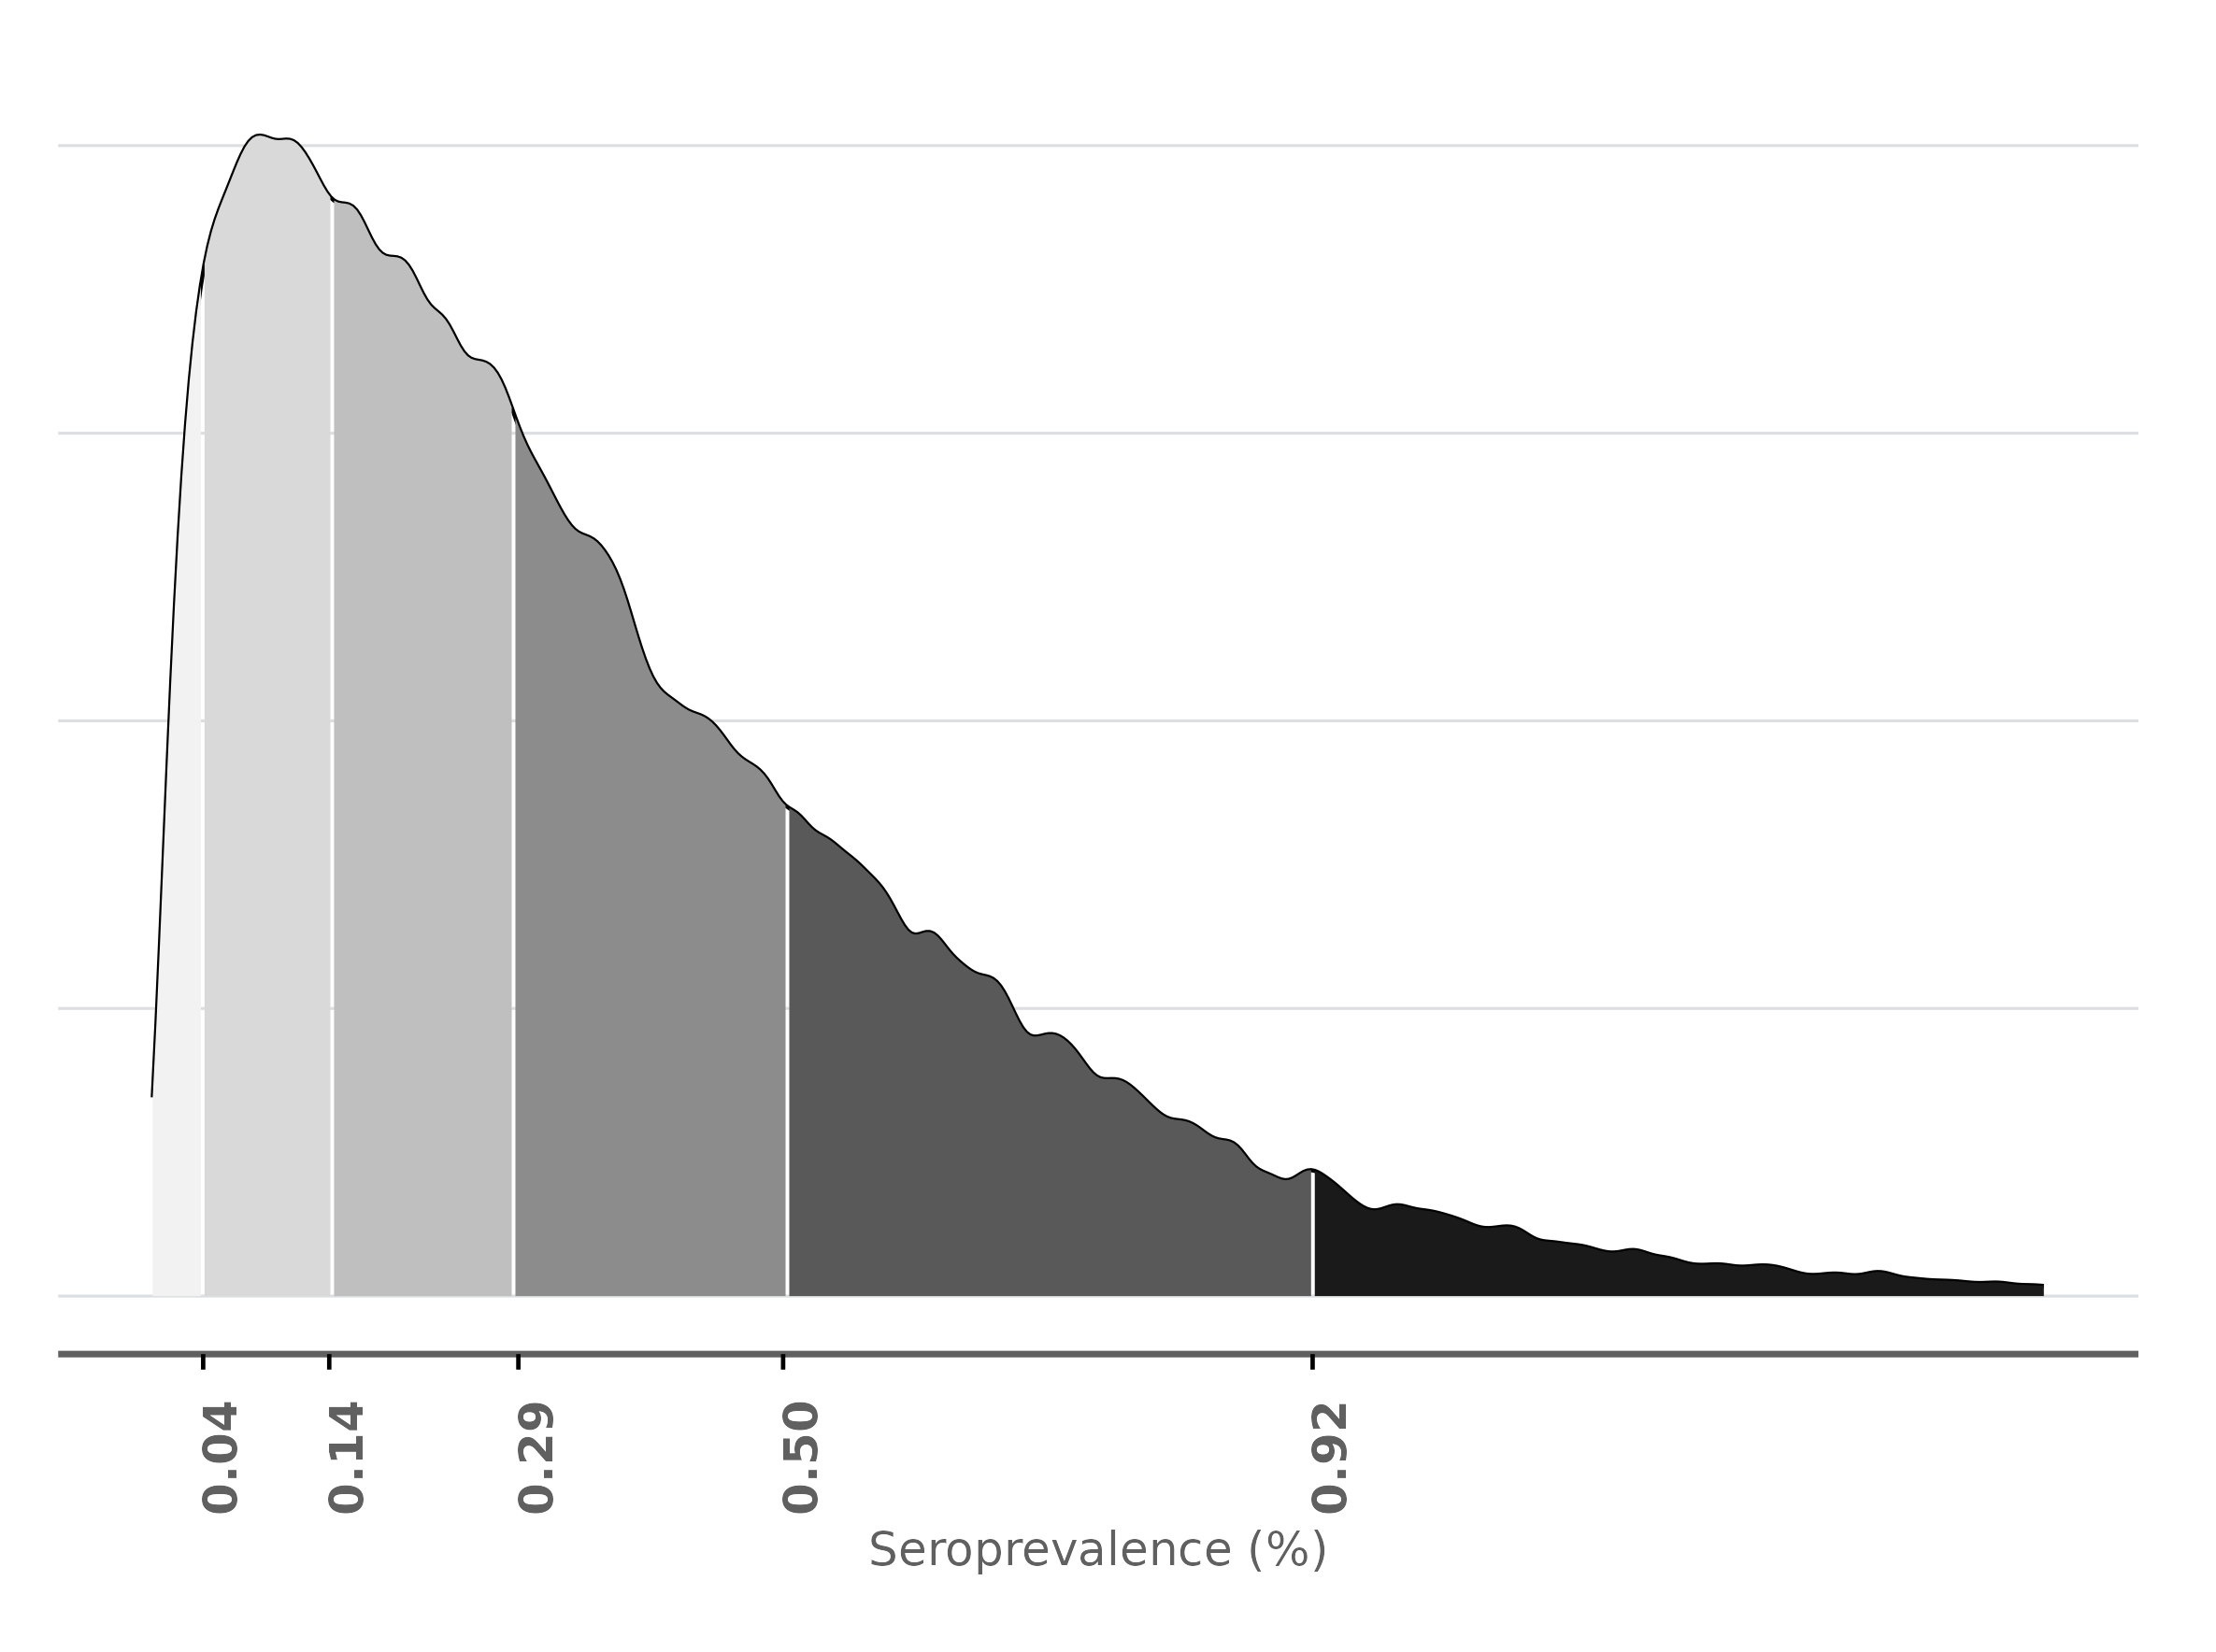
\includegraphics[width=\linewidth]{img/screen_p_sero_interestdate.png} 
\caption{Posterior density of $\pi^{(0)}(t)$, where $t$ corresponds to \printdate{2020-05-08}, learned from the screening test data.} \label{fig:screen_p_sero_interestdate}
\end{subfigure}%
\hspace*{\fill}
\begin{subfigure}{0.45\textwidth}
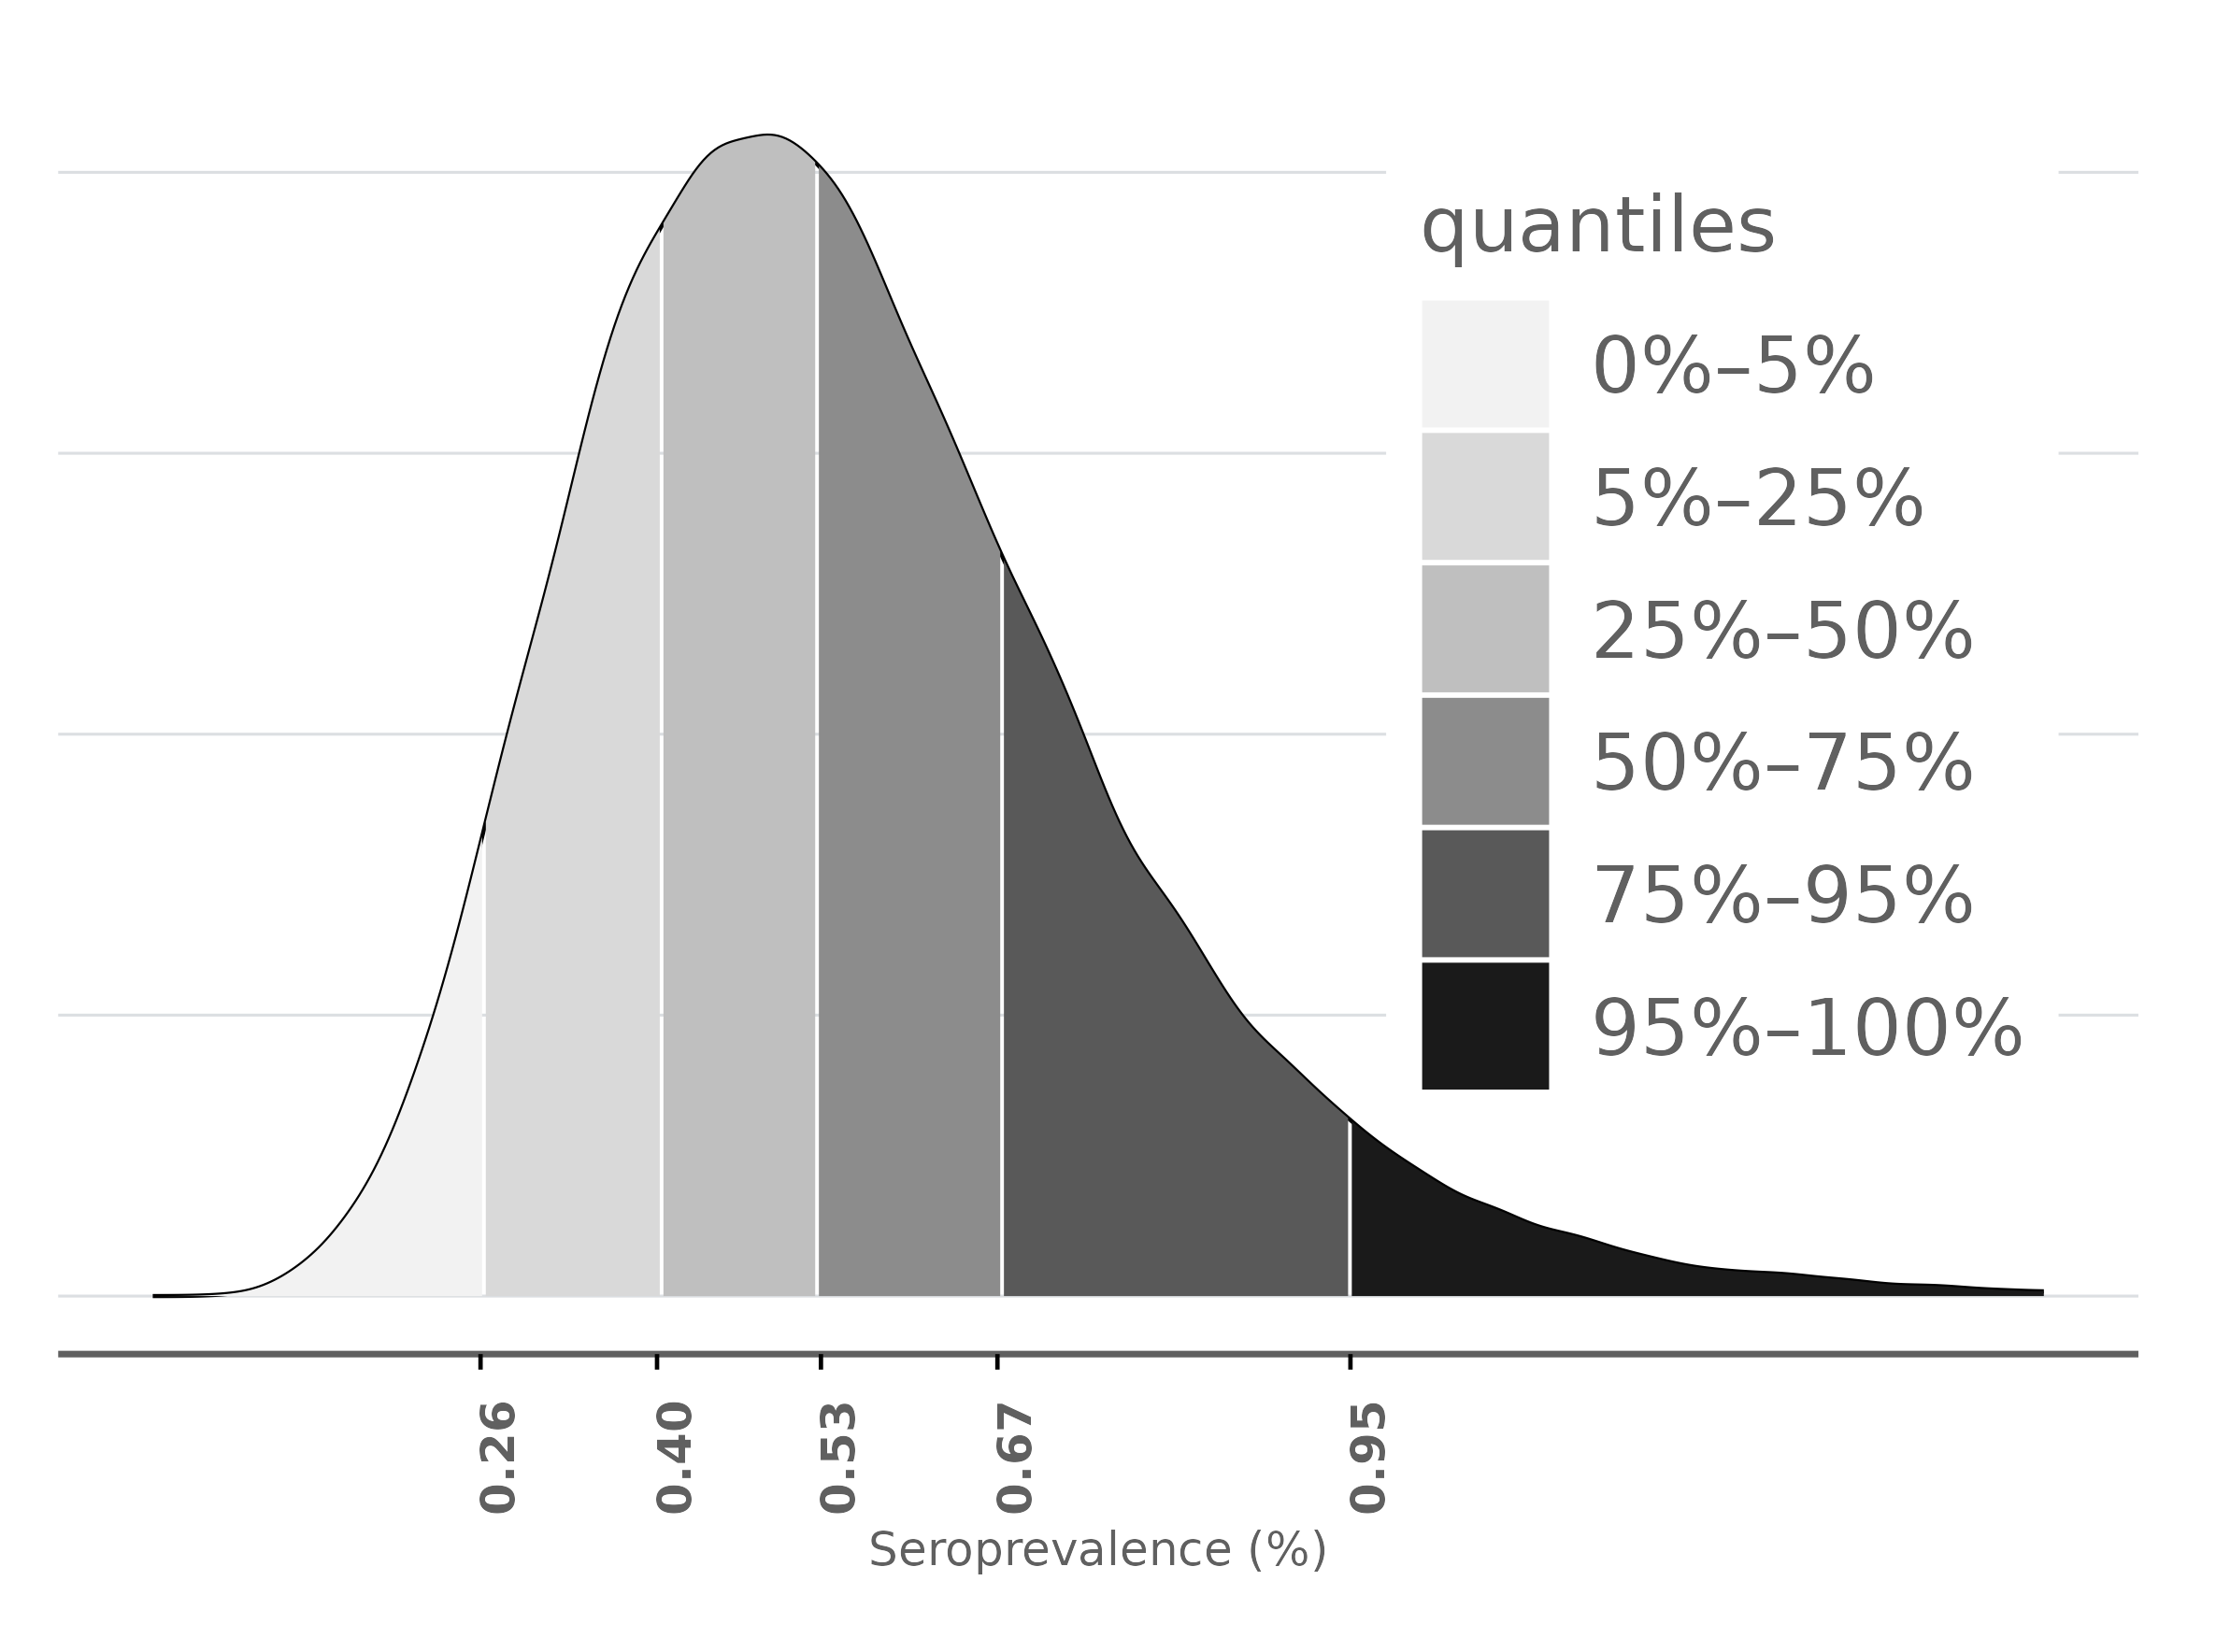
\includegraphics[width=\linewidth]{img/mnt_p_sero_interestdate.png}
\caption{Posterior density of $\pi^{(0)}(t)$, where $t$ corresponds to \printdate{2020-05-08}, learned from the confirmation test data.} \label{fig:mnt_p_sero_interestdate}
\end{subfigure}

\caption{Posterior distributions of seroprevalence $\pi^{(0)}(t)$, where t corresponds to \printdate{2020-05-08}, learned from the screening (left image) and confirmation (right image) test data. The seroprevalence is shown in percentage scale.}

\label{fig:results_interestdate_seroprev}
\end{figure}


\newpage



\begin{figure}[!htb]
\centering

\begin{subfigure}{0.47\textwidth}
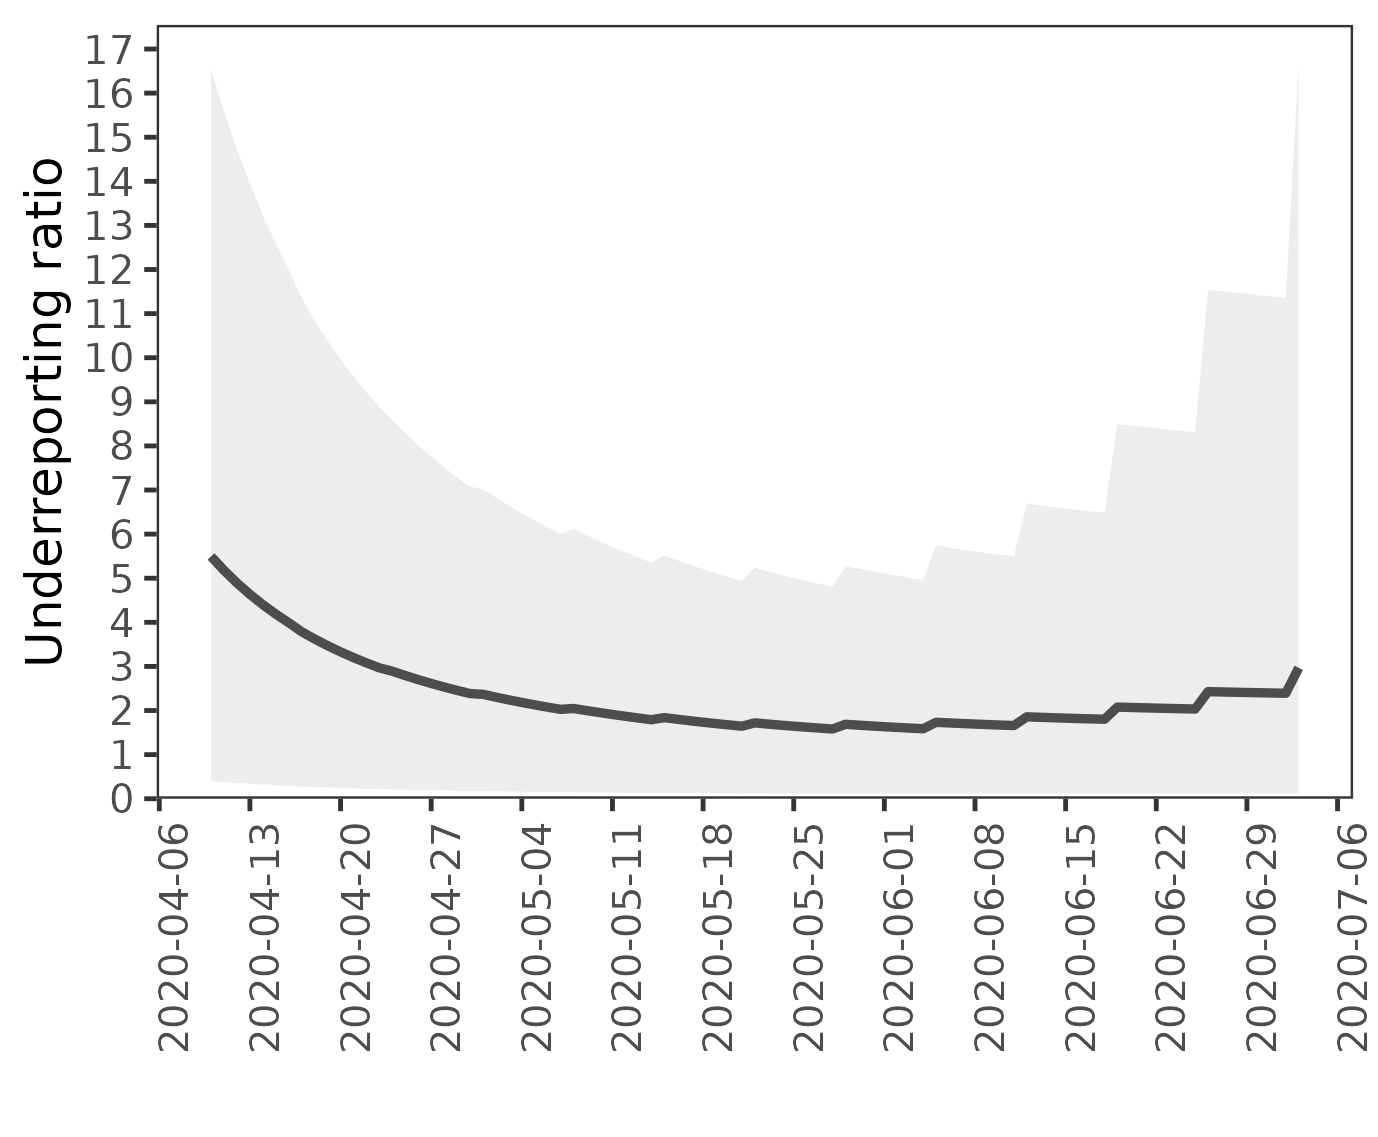
\includegraphics[width=\linewidth]{img/ttr_screen_ratio.png} 
\caption{Posterior means and 95\% credible intervals of underreporting ratio $\Delta(t)$ (Screening test)} \label{fig:ttr_screen_ratio}
\end{subfigure}%
\hspace*{\fill}
\begin{subfigure}{0.47\textwidth}
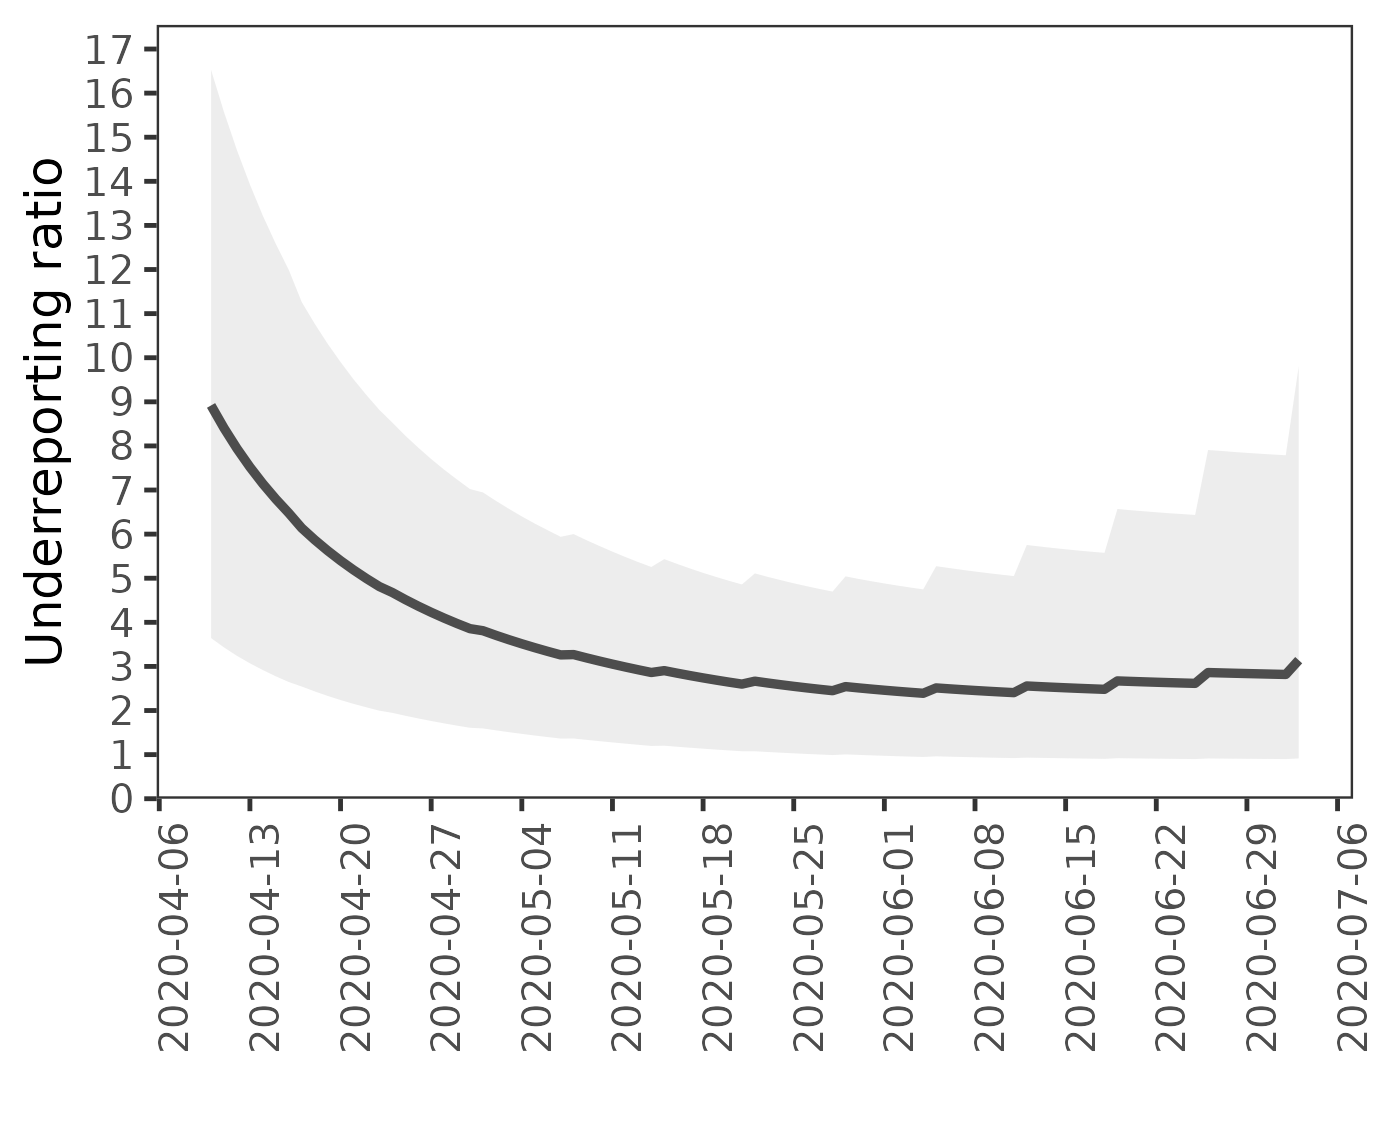
\includegraphics[width=\linewidth]{img/ttr_mnt_ratio.png}
\caption{Posterior means and 95\% credible intervals of underreporting ratio $\Delta(t)$ (Confirmation test)} \label{fig:ttr_mnt_ratio}
\end{subfigure}

\caption{Extent of underreporting in the extended capital region of Finland during the first wave of the COVID-19 epidemic. Both figures show the underreporting ratio $\Delta(t)$ (see equation \ref{eq:ratio}). The image on the left shows results for the screening test and the image on the right shows results for the confirmation test. Solid lines are posterior means and the shaded areas correspond to 95\% credible intervals derived from the pointwise 2.5\% and 97.5\% quantiles.}

\label{fig:underreporting}
\end{figure}


\newpage


\begin{figure}[!htb]
\centering

\begin{subfigure}{0.45\textwidth}
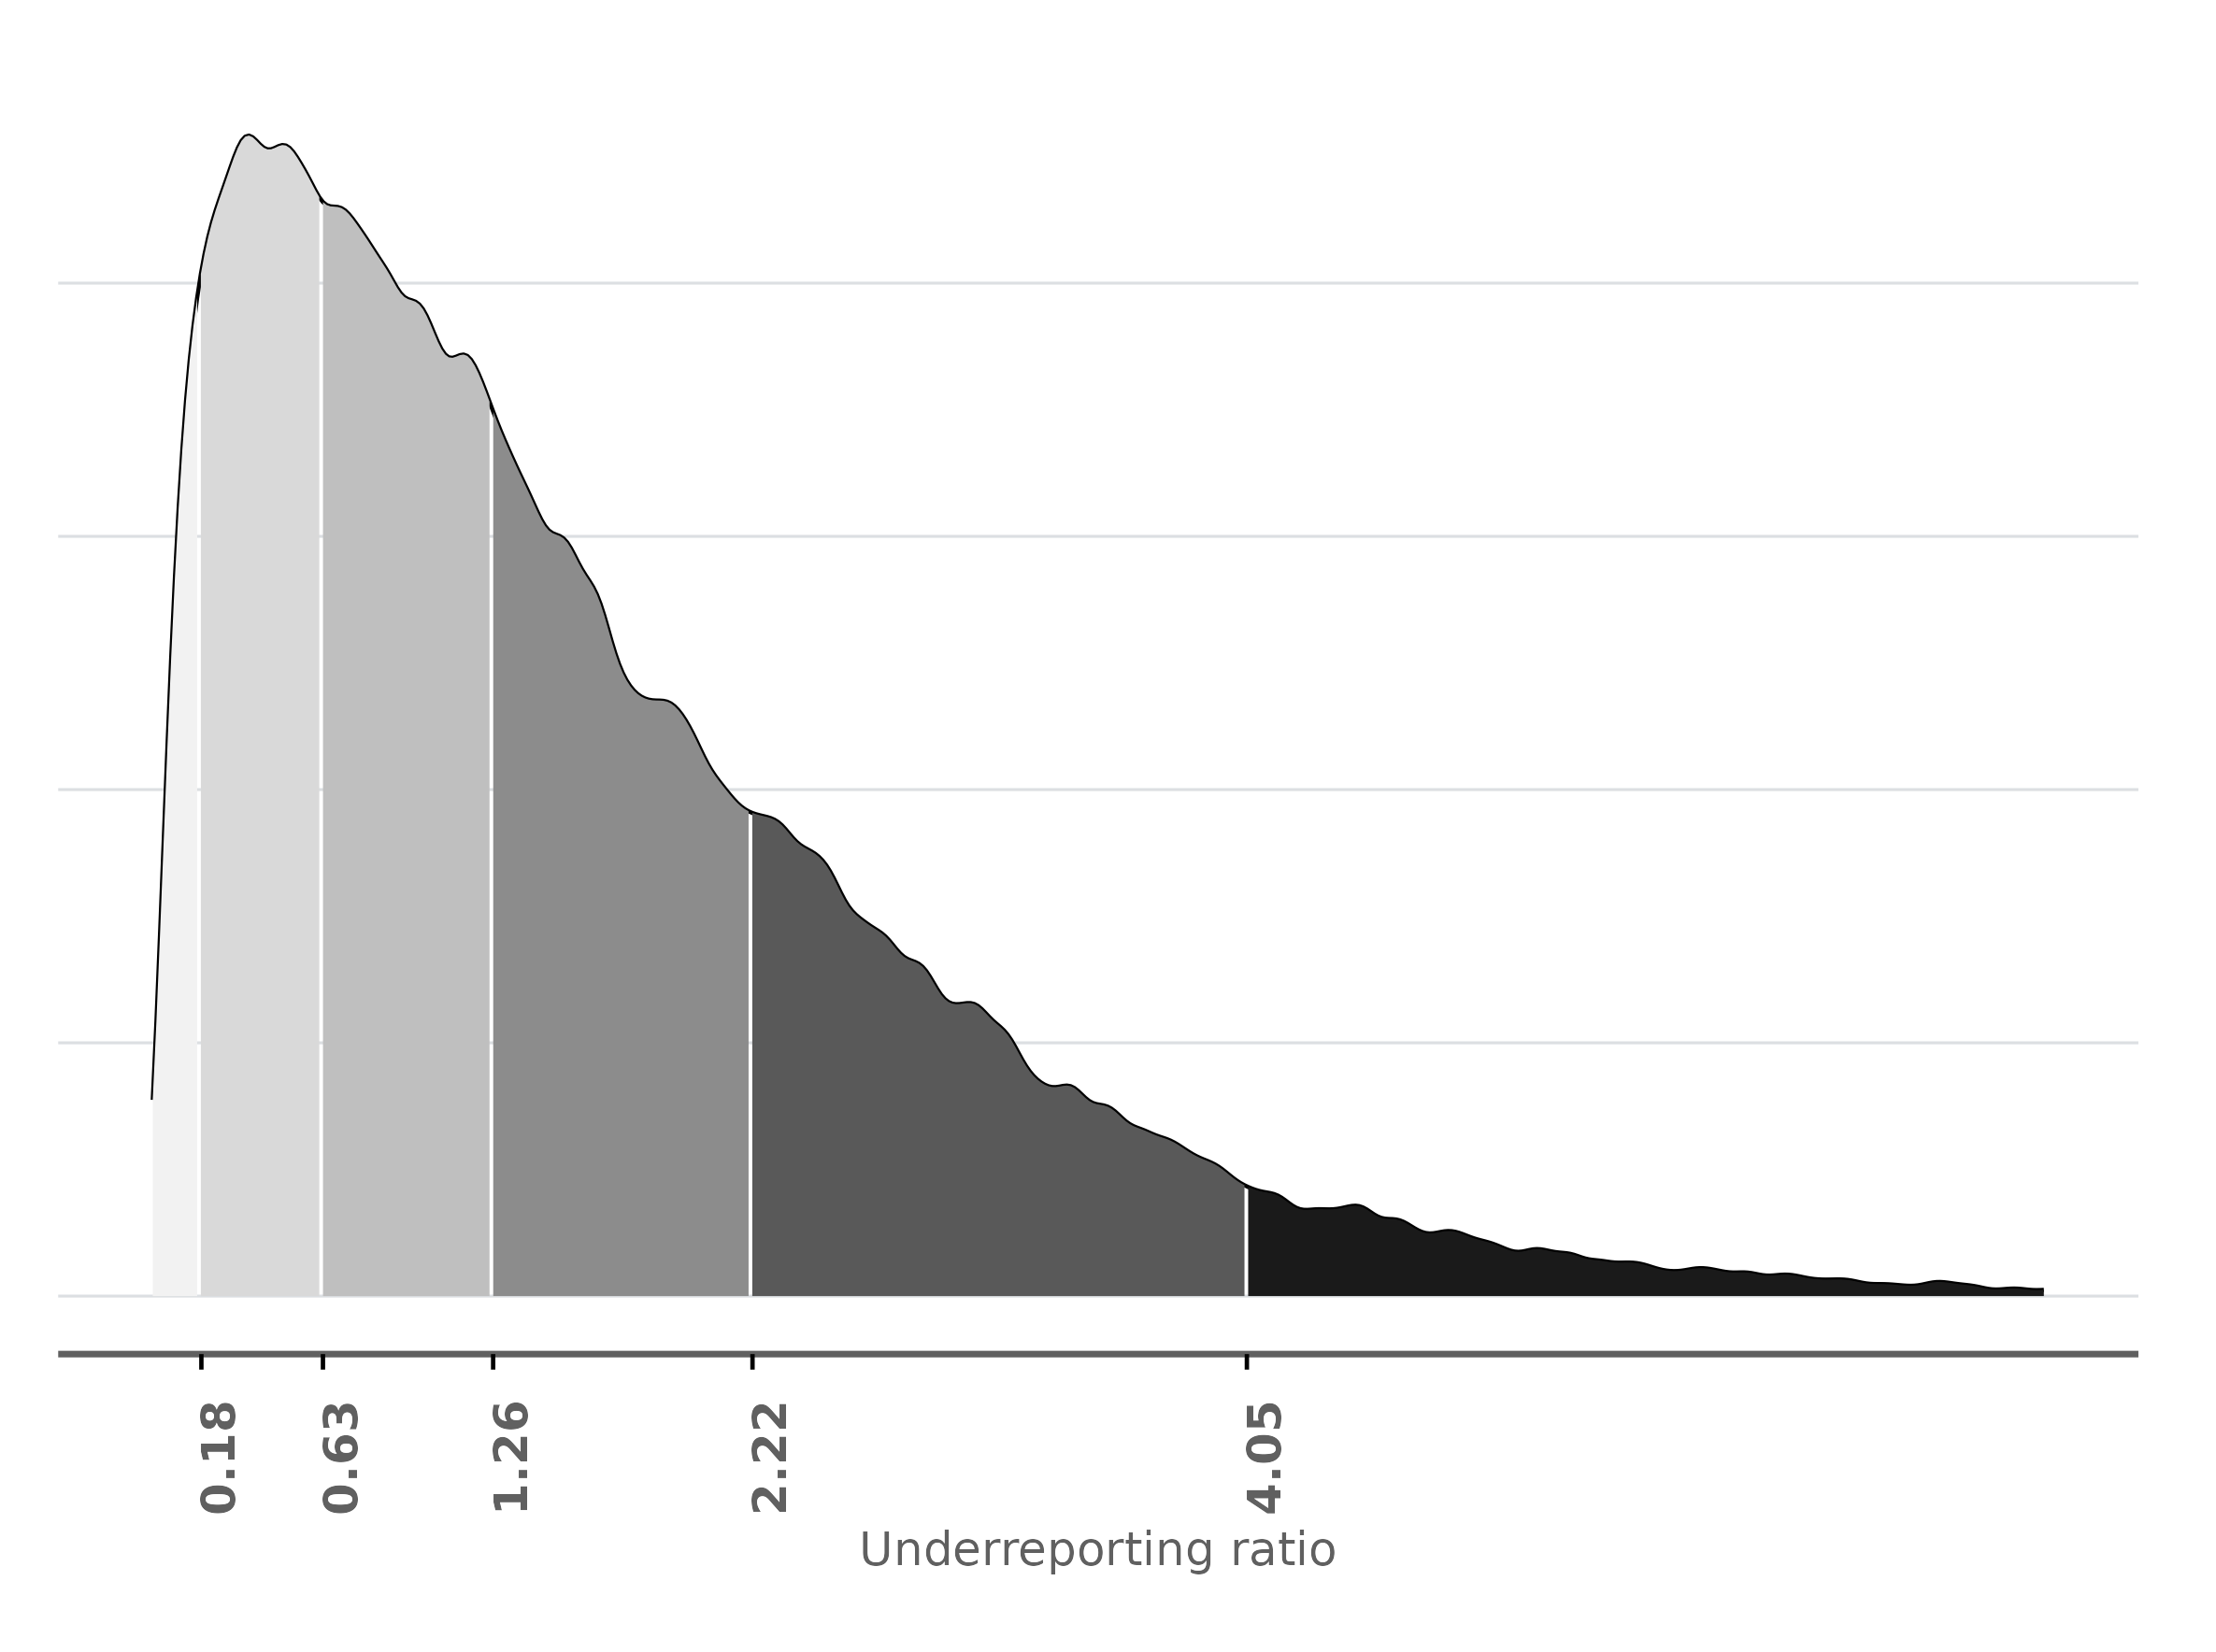
\includegraphics[width=\linewidth]{img/screen_ratio_interestdate.png}
\caption{Posterior density of $\Delta(t)$, where $t$ corresponds to \printdate{2020-05-08}, learned from screening test data}  \label{fig:screen_ratio_interestdate}
\end{subfigure}%
\hspace*{\fill}
\begin{subfigure}{0.45\textwidth}
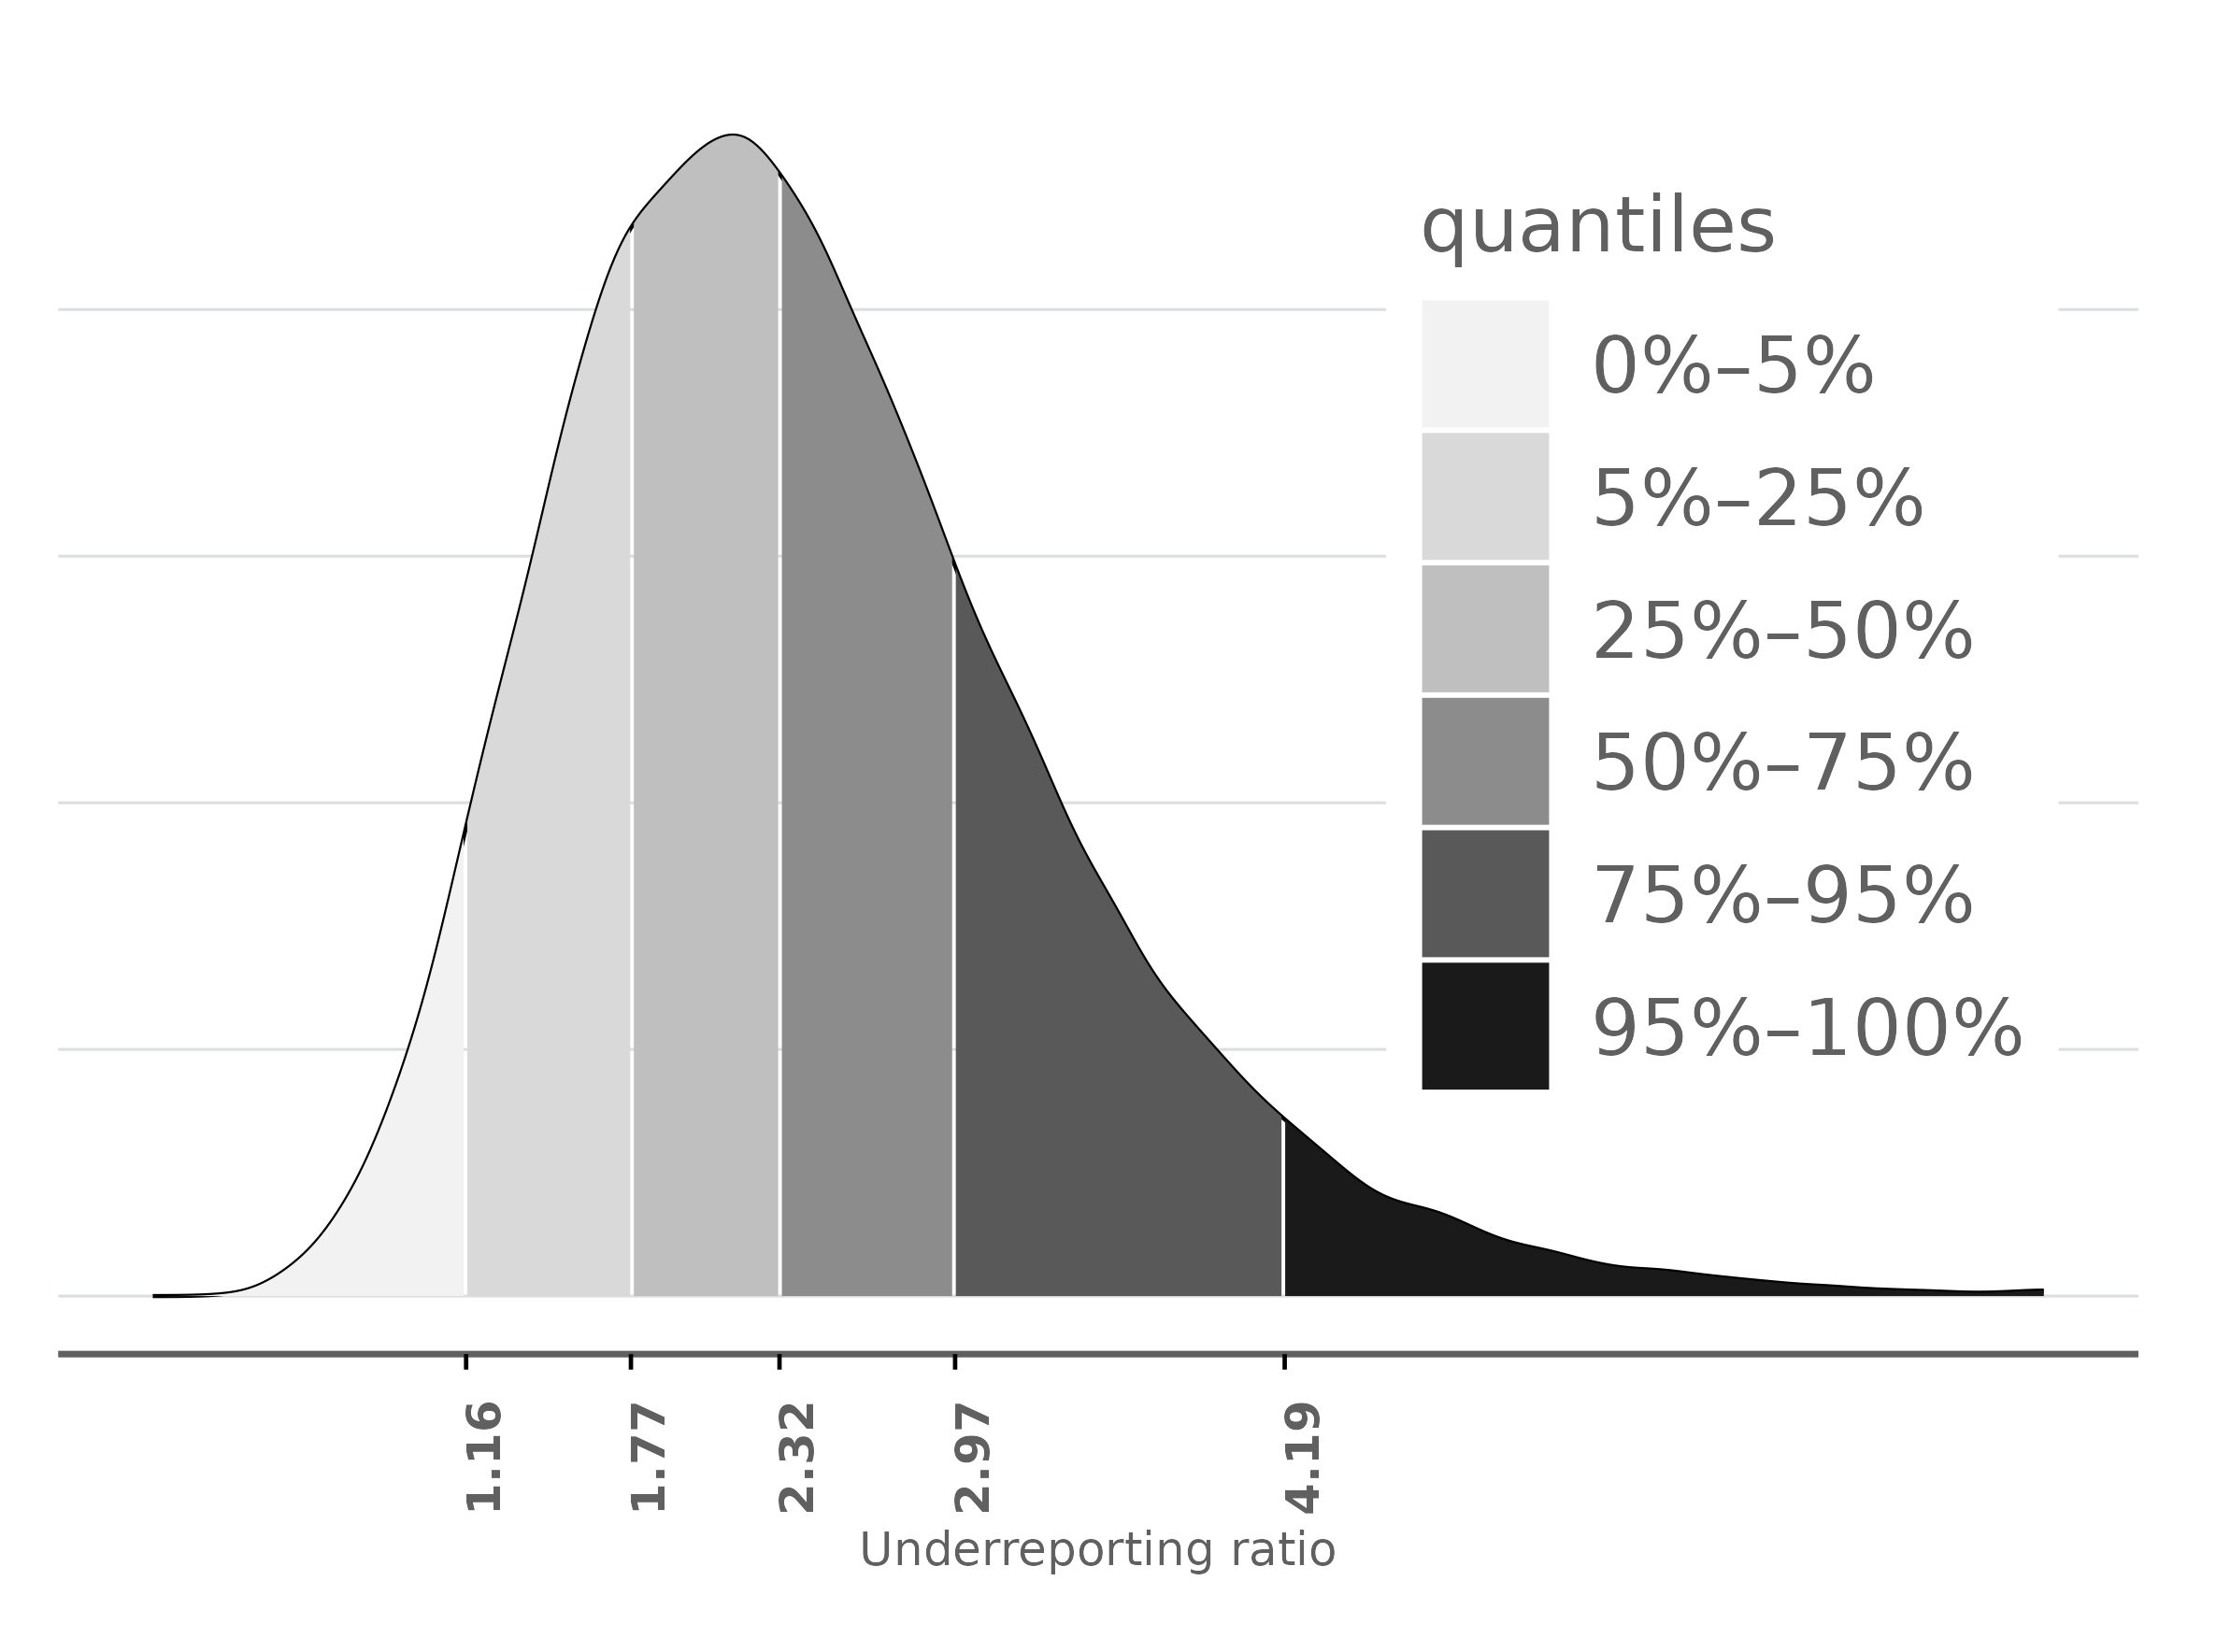
\includegraphics[width=\linewidth]{img/mnt_ratio_interestdate.png} 
\caption{Posterior density of $\Delta(t)$, where $t$ corresponds to \printdate{2020-05-08}0, learned from confirmation test data} \label{fig:mnt_ratio_interestdate}
\end{subfigure}

\caption{Posterior distributions of underreporting ratio $\Delta(t)$, where t corresponds to \printdate{2020-05-08}, learned from the screening test (left image) and confirmation test (right image) data.}

\label{fig:results_interestdate_ratio}
\end{figure}




\newpage




